% This is LLNCS.DEM the demonstration file of
% the LaTeX macro package from Springer-Verlag
% for Lecture Notes in Computer Science,
% version 2.4 for LaTeX2e as of 16. April 2010
%
\documentclass{llncs}
\usepackage{times}
\usepackage{graphicx}
\usepackage{epsf}
\usepackage{verbatim}
\usepackage{psfig}
\usepackage{cite}
\usepackage{url}
\usepackage{color}
\usepackage{alltt}

\usepackage{longtable,lscape}
\usepackage{slashbox,multirow}
\usepackage{colortbl}
\usepackage{mathrsfs}

\newcommand{\Add}{\CodeIn{add}}
\newcommand{\AVTree}{\CodeIn{AVTree}}
\newcommand{\Assignment}[3]{$\langle$ \Object{#1}, \Object{#2}, \Object{#3} $\rangle$}
\newcommand{\BinaryTreeRemove}{\CodeIn{BinaryTree\_remove}}
\newcommand{\BinaryTree}{\CodeIn{BinaryTree}}
\newcommand{\Caption}{\caption}
\newcommand{\Char}[1]{`#1'}
\newcommand{\CheckRep}{\CodeIn{checkRep}}
\newcommand{\ClassC}{\CodeIn{C}}
\newcommand{\CodeIn}[1]{{\small\texttt{#1}}}
\newcommand{\CodeOutSize}{\scriptsize}
\newcommand{\Comment}[1]{}
\newcommand{\Ensures}{\CodeIn{ensures}}
\newcommand{\ExtractMax}{\CodeIn{extractMax}}
\newcommand{\FAL}{field-ordering}
\newcommand{\FALs}{field-orderings}
\newcommand{\Fact}{observation}
\newcommand{\Get}{\CodeIn{get}}
\newcommand{\HashSet}{\CodeIn{HashSet}}
\newcommand{\HeapArray}{\CodeIn{HeapArray}}
\newcommand{\Intro}[1]{\emph{#1}}
\newcommand{\Invariant}{\CodeIn{invariant}}
\newcommand{\JUC}{\CodeIn{java.\-util.\-Collections}}
\newcommand{\JUS}{\CodeIn{java.\-util.\-Set}}
\newcommand{\JUTM}{\CodeIn{java.\-util.\-TreeMap}}
\newcommand{\JUTS}{\CodeIn{java.\-util.\-TreeSet}}
\newcommand{\JUV}{\CodeIn{java.\-util.\-Vector}}
\newcommand{\JMLPlusJUnit}{JML+JUnit}
\newcommand{\Korat}{Korat}
\newcommand{\Left}{\CodeIn{left}}
\newcommand{\Lookup}{\CodeIn{lookup}}
\newcommand{\MethM}{\CodeIn{m}}
\newcommand{\Node}[1]{\CodeIn{N}$_#1$}
\newcommand{\Null}{\CodeIn{null}}
\newcommand{\Object}[1]{\CodeIn{o}\ensuremath{_#1}}
\newcommand{\PostM}{\MethM$_{post}$}
\newcommand{\PreM}{\MethM$_{pre}$}
\newcommand{\Put}{\CodeIn{put}}
\newcommand{\Remove}{\CodeIn{remove}}
\newcommand{\RepOk}{\CodeIn{repOk}}
\newcommand{\Requires}{\CodeIn{requires}}
\newcommand{\Reverse}{\CodeIn{reverse}}
\newcommand{\Right}{\CodeIn{right}}
\newcommand{\Root}{\CodeIn{root}}
\newcommand{\Set}{\CodeIn{set}}
\newcommand{\State}[1]{2^{#1}}
\newcommand{\TestEra}{TestEra}
\newcommand{\TreeMap}{\CodeIn{TreeMap}}

\newenvironment{CodeOut}{\begin{scriptsize}}{\end{scriptsize}}
\newenvironment{SmallOut}{\begin{small}}{\end{small}}

\newcommand{\pairwiseEquals}{PairwiseEquals}
\newcommand{\monitorEquals}{MonitorEquals}
%\newcommand{\monitorWField}{WholeStateW}
\newcommand{\traverseField}{WholeState}
\newcommand{\monitorSMSeq}{ModifyingSeq}
\newcommand{\monitorSeq}{WholeSeq}

\newcommand{\IntStack}{\CodeIn{IntStack}}
\newcommand{\UBStack}{\CodeIn{UBStack}}
\newcommand{\BSet}{\CodeIn{BSet}}
\newcommand{\BBag}{\CodeIn{BBag}}
\newcommand{\ShoppingCart}{\CodeIn{ShoppingCart}}
\newcommand{\BankAccount}{\CodeIn{BankAccount}}
\newcommand{\BinarySearchTree}{\CodeIn{BinarySearchTree}}
\newcommand{\LinkedList}{\CodeIn{LinkedList}}

\newcommand{\Book}{\CodeIn{Book}}
\newcommand{\Library}{\CodeIn{Library}}

\newcommand{\Jtest}{Jtest}
\newcommand{\JCrasher}{JCrasher}
\newcommand{\Daikon}{Daikon}
\newcommand{\JUnit}{JUnit}

\newcommand{\trie}{trie}

\newcommand{\Perl}{Perl}


\newcommand{\SubjectCount}{11}
\newcommand{\DSSubjectCount}{two}

\newcommand{\Equals}{\CodeIn{equals}}
\newcommand{\Pairwise}{PairwiseEquals}
\newcommand{\Subgraph}{MonitorEquals}
\newcommand{\Concrete}{WholeState}
\newcommand{\ModSeq}{ModifyingSeq}
\newcommand{\Seq}{WholeSeq}
\newcommand{\Aeq}{equality}

\newcommand{\Meaning}[1]{\ensuremath{[\![}#1\ensuremath{]\!]}}
\newcommand{\Pair}[2]{\ensuremath{\langle #1, #2 \rangle}}
\newcommand{\Triple}[3]{\ensuremath{\langle #1, #2, #3 \rangle}}
\newcommand{\SetSuch}[2]{\ensuremath{\{ #1 | #2 \}}}

\newcommand{\Equiv}[2]{\ensuremath{#1 \EquivSTRel{} #2}}
\newcommand{\EquivME}{\Equiv}
\newcommand{\EquivST}{\Equiv}
\newcommand{\EquivSTRel}{\ensuremath{\cong}}
\newcommand{\Redundant}[2]{\ensuremath{#1 \lhd #2}}
\newcommand{\VB}{\ensuremath{\mid}}
\newcommand{\MES}{method-entry state}

\newcommand{\Small}[1]{{\small{#1}}}

\newcommand{\CenterCell}[1]{\multicolumn{1}{c|}{#1}}



\pagestyle{empty}
%\usepackage{latex8}
\usepackage{times}
\usepackage{algorithm}
\usepackage{algorithmic}
\usepackage{subfigure}
\usepackage{wrapfig}

%\usepackage{algorithm2e}

\usepackage{graphicx}
\usepackage{epsfig}
\usepackage{url}
%
\usepackage{makeidx}  % allows for indexgeneration
%
\begin{document}
%
\frontmatter          % for the preliminaries
%
\pagestyle{headings}  % switches on printing of running heads
\addtocmark{Hamiltonian Mechanics} % additional mark in the TOC


\mainmatter              % start of the contributions
%
\title{eXpress: Guided Path Exploration for Regression Test Generation}%
\titlerunning{eXpress}  % abbreviated title (for running head)
%                                     also used for the TOC unless
%                                     \toctitle is used
%
\author{Kunal Taneja\inst{1} \and Tao Xie\inst{1}
\and Nikolai Tillmann\inst{2} \and Jonathan de Halleux\inst{2} \and Wolfram Schulte\inst{2}}

\institute{Department of Computer Science, North Carolina State University, Raleigh, NC\\
\email{\{ktaneja,txie\}@ncsu.edu}
\and
Microsoft Research, One Microsoft Way, Redmond, WA\\
\email{\{nikolait, jhalleux, schulte\}@microsoft.com}
}
%\author{
%Kunal Taneja$^1$, \hspace{0.05in} Tao Xie$^1$,  \hspace{0.05in} Nikolai Tillmann$^2$,  \hspace{0.05in} Jonathan de Halleux$^2$,   \hspace{0.05in} Wolfram Schulte$^2$\\
%       \small{$^1$Department of Computer Science, North Carolina State University, Raleigh, NC}\\
%       \small{$^2$Microsoft Research, One Microsoft Way, Redmond, WA,}\\
%       \small{$^1$\{ktaneja, txie\}@ncsu.edu, $^2$\{nikolait, jhalleux, schulte\}@microsoft.com} 
%}   

\maketitle              % typeset the title of the contribution

\thispagestyle{empty}
\begin{sloppy}

\vspace{-1ex}
\begin{abstract}

Software developers often face
challenges in reusing open source frameworks due to several factors
such as the framework complexity and lack of proper
documentation. In this paper, we propose a code-search-engine-based
approach that detects \Intro{hotspots} in a given framework
by mining code examples gathered from open source repositories available on the web; 
these hotspots are API classes and methods that are frequently reused. 
Hotspots can serve as starting points for developers
in understanding and reusing the given framework. 
Our approach also detects \Intro{coldspots}, which are API classes and methods that are rarely used.
Coldspots serve as caveats for developers as there can 
be difficulties in finding relevant code examples and are generally less exercised
compared to hotspots. We developed a tool, called SpotWeb, for
frameworks or libraries written in Java and used our tool
to detect hotspots and coldspots of eight widely used open source
frameworks. We show the utility of our detected hotspots 
by comparing these hotspots with the API classes reused by a real application
and compare our results with the results of a previous related approach.
\end{abstract}


\section{Introduction}
\label{sec:intro}
Regression test generation aims at generating a test suite that can detect behavioral differences between the original and the new versions of a program. A behavioral difference between two versions of a program can be reflected by the difference between the observable outputs produced by the execution of the same test (referred to as a difference-exposing test) on the two versions. Developers can inspect these behavioral differences to determine whether they are intended or unintended (i.e., regression faults).

Regression test generation can be automated by using Dynamic Symbolic
Execution (DSE)~\cite{dart, cute, exe}, a state-of-the-art test generation
technique, to generate a test suite achieving high
structural coverage. DSE explores paths in a program to
achieve high structural coverage, and exploration of all
these paths can often be expensive. However, if our aim is
to detect behavioral differences between two versions of a
program, we do not need to explore all these paths in the program
since not all these paths are relevant for detecting behavioral
differences.

To formally investigate irrelevant paths for exposing behavioral differences, we adopt the 
Propagation, Infection, and Execution (PIE) model~\cite{voas} of error propagation. According to the PIE model, a fault can be detected by a test if a faulty statement is executed (E), the execution of the faulty statement infects the state (I), and the infected state (i.e., error) propagates to an observable output (P). A change in the new version of a program can be treated as a fault and then the PIE model is applicable for effect propagation of the change. Many paths in a program often cannot help in satisfying any of the conditions P, I, or E of the PIE model. 

In this paper, we present an approach{\footnote{\scriptsize{An earlier version of this work~\cite{taneja09:guided} is described in a four-page paper that appears in the NIER track of ICSE 2009. This
version significantly extends the previous work in the following major ways.
First, in this paper, we develop techniques for efficiently finding irrelevant branches 
that cannot execute any change. 
Second, we develop techniques for exploiting the existing test suite for efficiently generating regression tests.
Third, we automate our approach by developing a tool.
Fourth, we conduct extensive experiments to evaluate our approach.}} \CodeIn{eXpress} and its implementations that uses DSE to detect behavioral differences based on the notion of the PIE model.

Our approach first determines all the branches (in the program under test) that cannot help in achieving any of the conditions E and I of the PIE model in terms of the changes in the program. To make test generation efficient, we develop a new search strategy for DSE to avoid exploring these irrelevant branches (including which can lead to an irrelevant path\footnote{\scriptsize{An irrelevant path is a path that cannot help in achieving P, I, and E of the PIE model.}}). In particular, our approach guides DSE to avoid from flipping branching nodes\footnote{\scriptsize{A branching node in the execution tree of a program is an instance of a conditional statement in the source code. A branching node consists of two sides (or more than two sides for a \CodeIn{switch} statement): the true branch and the false branch. Flipping a branching node is flipping the execution of the program from the true (or false) branch of the branching node to the false (or true) branch. Flipping a branching node representing a switch statement is flipping the execution of the current branch to another unexplored branch.}}, which on flipping execute some irrelevant branch. 

In addition, our approach can exploit the existing test suite (if available) for the original version by seeding the tests in the test suite to the program exploration. Our technique of seeding the exploration with the existing test suite can be used to efficiently augment an existing test suite so that various changed parts of the program (that are not covered by the existing test suite) are covered by the augmented test suite. 

\Comment{In addition, our approach prioritizes the flipping of branching nodes\footnote{A branching node in the execution tree of a program is an instance of a conditional statement in the source code. A branching node consists of two sides (or more than two sides for a \CodeIn{switch} statement): the true branch and the false branch. Flipping a branching node is flipping the execution of the program from the true (or false) branch of the branching node to the false (or true) branch.  Flipping a branching node representing a switch statement is flipping the execution of current branch to some unexplored branch.} in such a manner that behavioral differences are more likely to be detected earlier in path exploration.
}

This paper makes the following major contributions:
\\ \textbf{Path Exploration for Regression Test Generation.} We propose an approach called \CodeIn{eXpress} that uses DSE for efficient generation of regression unit tests. To the best
of our knowledge, ours is the first approach that guides path exploration on the new version specifically for regression test generation.
\\ \textbf{Incremental Exploration.} We develop a technique for exploiting an existing test suite, so that path exploration focuses on covering the changes rather than starting from scratch. To the best of our knowledge, ours is the first technique that leverages an existing test suite for automated regression test generation.
\\ \textbf{Implementation.} We have implemented our \CodeIn{eXpress} approach in a tool as an extension for Pex~\cite{Pex},  an automated structural testing tool for .NET developed at Microsoft Research. Pex has been previously used internally at Microsoft to test core components of the .NET architecture and has found serious
bugs~\cite{Pex}. The current Pex has been downloaded for thousands of times in industry. 
\\ \textbf{Evaluation.} We have conducted experiments on 72 versions (in total) of four programs. Experimental results show that our approach requires about 53\% fewer runs (i.e., explored paths) on average to cause the execution of a changed region and 44\% fewer to cause program-state differences after its execution than exploration without guidance. In addition, our approach requires 71\% fewer runs to cover all the changed regions (i.e, infection) by exploiting an existing test suite than exploration without using the test suite. 
%\end{itemize}
\Comment{
The rest of the paper is organized as follows. Section~\ref{sec:example} 
presents an example to illustrate our approach. Section~\ref{sec:approach} presents 
our approach and the major components involved in the approach. Section~\ref{sec:evaluation}
presents the evaluation results. Section~\ref{sec:validity} discusses the threats to validity of the evaluation results. Section~\ref{sec:related} discusses related
work. Section~\ref{sec:discussion} discusses research issues and future work,
and Section~\ref{sec:conclusion} concludes.
}
\section{Background}
\label{sec:background}

We next provide details of two major concepts used in the rest of
the paper: dynamic symbolic execution and dynamic code coverage.

%-----------------------------------------------------------------------------
\subsection{Dynamic Symbolic Execution}

In our approach, we use Pex as an example state-of-the-art dynamic symbolic 
execution tool. Pex~\cite{tillman:pexwhite} is an automatic unit-test-generation 
tool developed by Microsoft. Pex accepts PUTs as input and generates conventional 
unit tests that can achieve high 
structural coverage of the code under test. Initially, Pex
executes the code under test with random inputs. While executing
the code under test, Pex collects constraints on inputs from predicates
in branching statements. Pex next solves collected constraints
to generate new test inputs that guide future executions along
new paths. Pex includes various optimization techniques such as
reducing the size of the formula before giving it over constraint solver.

%-----------------------------------------------------------------------------
\subsection{Dynamic Code Coverage}

In this paper, we use Pex generated reports for measuring coverage. These coverage
reports are called dynamic, because Pex knows only about the code that was already executed.
As Pex is not aware of the code that is not yet executed, dynamic code coverage
cannot give absolute values for the coverage. The primary reason for using
dynamic code coverage in our paper is that C\# allows generate code during run time.
Therefore, it is often not possible to find out how much code exists beforehand.
\section{Example}
\label{sec:example}
In this section, we illustrate our \CodeIn{eXpress} approach with an example. \CodeIn{eXpress} takes as input two versions of a program and produces as output a regression test suite, with the objective of detecting behavioral differences (if any exist) between the two versions of program under test. Although \CodeIn{eXpress} analyzes assembly code of C\# programs, in this section, we illustrate the \CodeIn{eXpress} approach using program source code. 

    \begin{figure}[t]
    \centering
        %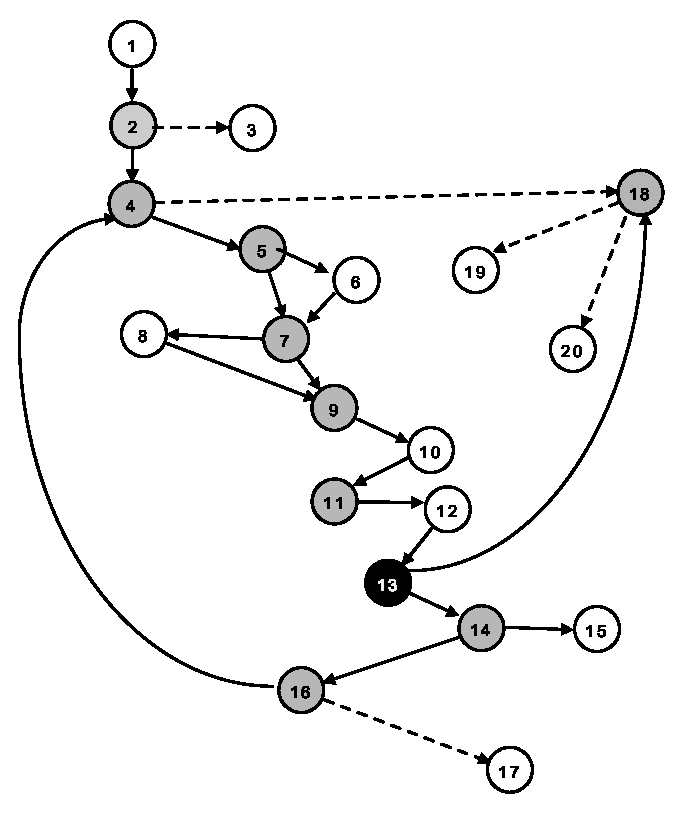
\includegraphics[width=6cm, keepaspectratio]{Figures/cfg3}
         \subfigure{\includegraphics[width=12.5cm, keepaspectratio]{Figures/example}}
         
    \vspace{-0.6cm}
    \caption{\scriptsize{An example program on the left side and the instrumented program on the right.}}
    \label{fig:example}
     \vspace{-0.7cm}
    \end{figure}
    
%\begin{figure}[t]
%
%%\begin{subfigure}
%\begin{CodeOut}
%\begin{alltt}
%
%  \hspace{0.25cm}\textbf{static public int} TestMe(\textbf{char[] }c, \textbf{int} n)\{
%1 \hspace{0.5cm} \textbf{int} state = 0;
%2 \hspace{0.5cm} \textbf{if}(c == \textbf{null} || c.Length == 0) 
%3 \hspace{0.75cm} \textbf{return -1;}   
%4 \hspace{0.5cm} \textbf{for}(\textbf{int} i=0; i< c.Length; i++)\{
%5 \hspace{1.0cm} \textbf{if}(c[i] == "[") state =1;
%6 \hspace{1.0cm} \textbf{else if}(state == 1 && c[i] == "\{") state =2;
%7 \hspace{1.0cm} \textbf{else if}(state == 2 &&  c[i] == "<") state =3;
%8 \hspace{1.0cm} \textbf{else if}(state == 3 && c[i] == "*")\{ 
%9 \hspace{1.25cm} state =4;
%10\hspace{1.25cm} \textbf{if}(c.Length==15) 
%11\hspace{1.5cm} state = state + n;//Added in new version
%	\hspace{1.0cm}   \}
%12\hspace{1.0cm} \textbf{if}(c[i]==' ') 
%13\hspace{1.25cm} \textbf{return};
%14\hspace{1.0cm} \textbf{if}(!(c[i] >= 'a' && c[i] <= 'z')\{
%15\hspace{1.25cm} state=-1; \textbf{return};
%  \hspace{1.0cm} \}
%  \hspace{.75cm} \}
%  \hspace{.50cm} \}
%16\hspace{.50cm} \textbf{if}(c[15] == '\}')
%17\hspace{.70cm} \textbf{return} state;
%18\hspace{.5cm} \textbf{return} -1;
%  \hspace{0.25cm}\}
%  
%\end{alltt}
%\end{CodeOut}
%\vspace{-0.9 cm}
%\caption{An example program}
%\label{fig:example}
%%\end{subfigure}
%
%\end{figure}
%
%\begin{figure}[t]
%\begin{CodeOut}
%\begin{alltt}
%
%  \hspace{0.25cm}\textbf{static public int} fOld(\textbf{int }state, 
%  \hspace{0.5cm}\textbf{int} length, \textbf{int} n)\{
%1 \hspace{0.5cm} \textbf{return} state;
%  \hspace{0.25cm}\}
%  
%  \hspace{0.25cm}\textbf{static public int} fNew(\textbf{int }state,
%  \hspace{0.5cm}\textbf{int} length, \textbf{int} n)\{
%1 \hspace{0.5cm} \textbf{if}(c.Length==15) state = state + n;
%2	\hspace{0.5cm} \textbf{return} state;
%  \hspace{0.25cm}\}
%  
%  \hspace{0.25cm}\textbf{static public int} TestMe(\textbf{char[] }c, \textbf{int} n)\{
%  \hspace{0.5cm} ...
%10\hspace{0.5cm} \textbf{int} stateCopy = state;
%11\hspace{0.5cm} state = fNew(state, c.Length, n);
%12\hspace{0.5cm} stateCopy = fOld(stateCopy, c.Length, n);
%13\hspace{0.5cm} if(state != stateCopy);   //Infection Condition
%  \hspace{0.5cm} ...
%  \hspace{0.25cm}\}
%\end{alltt}
%\end{CodeOut}
%\caption{Instrumentation to efficiently and effectively achieve I of the PIE model.}
%\vspace{-0.7 cm}
%\label{fig:example}
%\end{figure}


Consider the example in Figure~\ref{fig:example}. 
The left side of the figure shows a program \CodeIn{TestMe}. Lines 10 and 11 of the program are added in a new version.
\\ \textbf{Finding Irrelavant Branches.} 
%\CodeIn{eXpress} first compares the two program versions to find that Line 13 is added in the new version. \CodeIn{eXpress} then builds a Control-Flow Graph (CFG) of new version of  the program under test and marks the changed vertices in the graph.
The left side of Figure~\ref{fig:Tree} shows the CFG of the program in Figure~\ref{fig:example}. The labels of vertices in the CFG denote the corresponding line numbers in Figure~\ref{fig:example}. The black vertex denotes the newly added statements at Lines 10 and 11. The gray vertices denote the branching nodes (for the branching statements in the program), while the white vertices denote the other statements in the program. From the CFG, \CodeIn{eXpress} finds the following categories of branches.
%\\ \textbf{Difference Finder.} The Difference Finder component compares the original and the new versions of the program under test to find differences between each corresponding method of the two program versions. For the program in Figure~\ref{fig:example}, Difference Finder detects that the statements at Line 13 are added in the new version. 
%\\ \textbf{Graph Builder. }The Graph Builder component then builds a Control-Flow Graph (CFG) of the new version of  the program under test and marks the changed vertices in the graph. Figure~\ref{fig:CFG} shows the CFG of the program in Figure~\ref{fig:example}. The labels of vertices in the CFG denote the corresponding line numbers in Figure~\ref{fig:example}. The black vertex denotes the newly added statements at Line 13. The gray vertices denote the branching nodes (for the branching statements in the program), while the white vertices denote the other statements in the program.
%\\ \textbf{Graph Traverser.} The Graph Traverser component traverses the CFG to find each branch\footnote{\scriptsize{A branch is an outgoing edge of a branching node.}} $b$ in a program such that if $b$ is taken, the program execution cannot help in finding behavioral differences between the original and the new program versions. These branches are used by the Dynamic Test Generator component to efficiently find behavioral differences between the original and new program version.
%In particular, the Graph Traverser finds two categories of branches.
\begin{itemize}
\vspace{-1ex}
\item \textbf{Category $B_{E+I}$.} On traversing the CFG in Figure~\ref{fig:Tree}, \CodeIn{eXpress} detects that taking the branches $<$$2, 3$$>$\footnote{\scriptsize{$<$$x,y$$>$ represents a branch from source vertex $x$ to destination vertex $y$}}, $<$$4, 16$$>$, $<$$16, 17$$>$, $<$$16, 18$$>$, $<$$12, 13$$>$ and $<$$14, 15$$>$ (dotted edges in Figure~\ref{fig:Tree}), the program execution cannot reach any of the black vertices. Hence, the execution of these branches cannot help in executing the changed statements or infecting the program state. \\ 
\vspace{-1ex} 
\item \textbf{Category $B_{P}$.} In addition, \CodeIn{eXpress} finds out that 
among the source vertices of the six branches in Category $B_{I+E}$, there is no path from any of the 
black vertices to vertex 3. Hence, a state infection after the execution of the black vertex 
cannot propagate through the branch $<2,3>$.
\end{itemize}
\vspace{-0.2cm}
\textbf{Instrumentation for State Infection.}
A DSE-based test generation tool tries to execute all feasible branches in the program. However the execution of 
all branches is not sufficient for infecting the program state. For example, 
a test generation tool can 
cover all the branches of \CodeIn{}TestMe (left side of Figure~\ref{fig:example}) with $n=0$ (a default input used by some tools) but to infect the program state, the tool
need to generate a nonzero value of $n$.
To guide the test generation tool to effectively achieve state infection,
\CodeIn{eXpress} instruments the new program version.
In particular, \CodeIn{eXpress} invokes the changed regions\footnote{\scriptsize{A changed region (in a new or modified program version) is a minimal set of statements that contains all modified (in new or original program version), added (in new program version), or deleted (in original program version) statements in a method. The changed region for the new program version in \CodeIn{TestMe} on the left side of Figure~\ref{fig:example} is shown in rectangular box, while the changed region of the original program version is empty.}} 
from the two program versions (with same inputs) and 
compares the outputs of the two changed regions. 
\CodeIn{eXpress} inserts branches in the new program version that are executed only 
when the outputs of the executions of the changed regions differ, i.e., when program
state is infected after the execution of the changed regions.

The right side of Figure~\ref{fig:example} shows the instrumented version of \CodeIn{TestMe} on the left side of 
Figure~\ref{fig:example}. 
\CodeIn{eXpress} identifies $state$, $length$, and $n$ as the inputs to the two changed regions
and $state$ as the output to the two changed regions.
\CodeIn{eXpress} then extracts the
changed regions in the original and new program versions as separate methods 
(\CodeIn{fOld} and \CodeIn{fNew}, respectively).
The parameters of the two methods are same as the identified inputs, while the return values 
are same as the identified output.
%The method \CodeIn{fOld} shows the method extracted for the old program version,
%while the method \CodeIn{fNew} shows the method extracted for the new program version.
%Since the changed region in the old program version is empty, the method \CodeIn{fOld} just 
%returns $state$,
%while the method \CodeIn{fNew} contains Lines 10 and 11 (of \CodeIn{TestMe} on the 
%left side of Figure~\ref{fig:example}) and returns the resulting value of $state$.
\CodeIn{eXpress} replaces the changed region of the new version of
\CodeIn{TestMe} by the invocation of the methods \CodeIn{fOld} and \CodeIn{fNew} 
(Lines 11 and 12 on the right side of Figure~\ref{fig:example}). 
Note that the variable $stateOld$ passed to 
\CodeIn{fOld} is a copy of the variable $state$ passed to \CodeIn{fNew} (Line 10 on the right side of ~\ref{fig:example}) because 
$state$ may be updated by \CodeIn{fNew} since $state$ is also an output of the changed regions. 
\CodeIn{eXpress} then inserts an \CodeIn{if} statement (Line 13 on the right side of Figure~\ref{fig:example})
in the program comparing the outputs of the two methods.
Note that the outputs of the two methods are different if and only if the program state is infected.
A DSE-based test generation tool determines that it needs to generate inputs 
satisfying \CodeIn{c.Length == 15 AND state != state + n} to cover the true branch of the added \CodeIn{if} statement. 
Hence, the tool generates a nonzero value of $n$ to satisfy the constraint and infect the program state. 
\begin{figure}[t]
    \centering
        %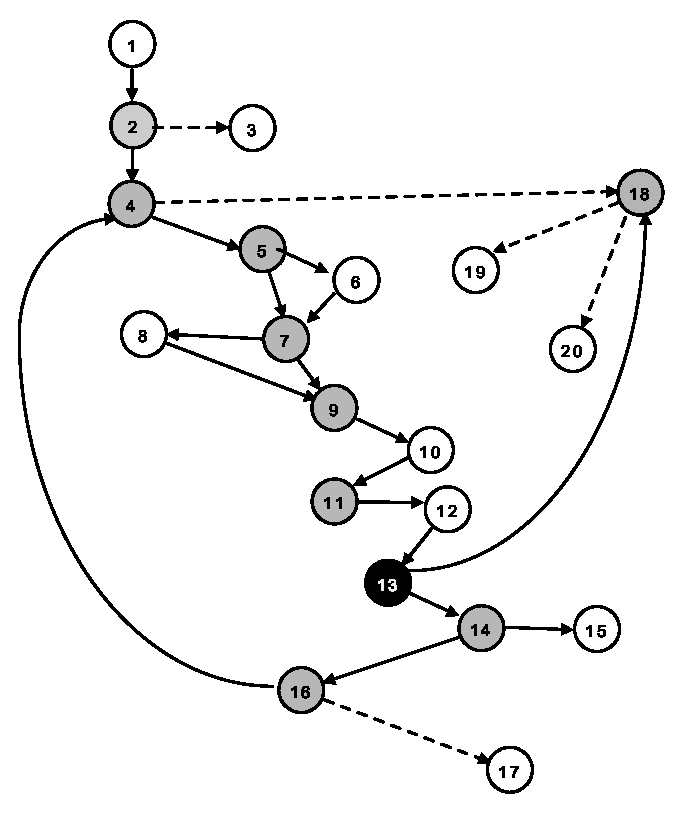
\includegraphics[width=6cm, keepaspectratio]{Figures/cfg3}
         \subfigure{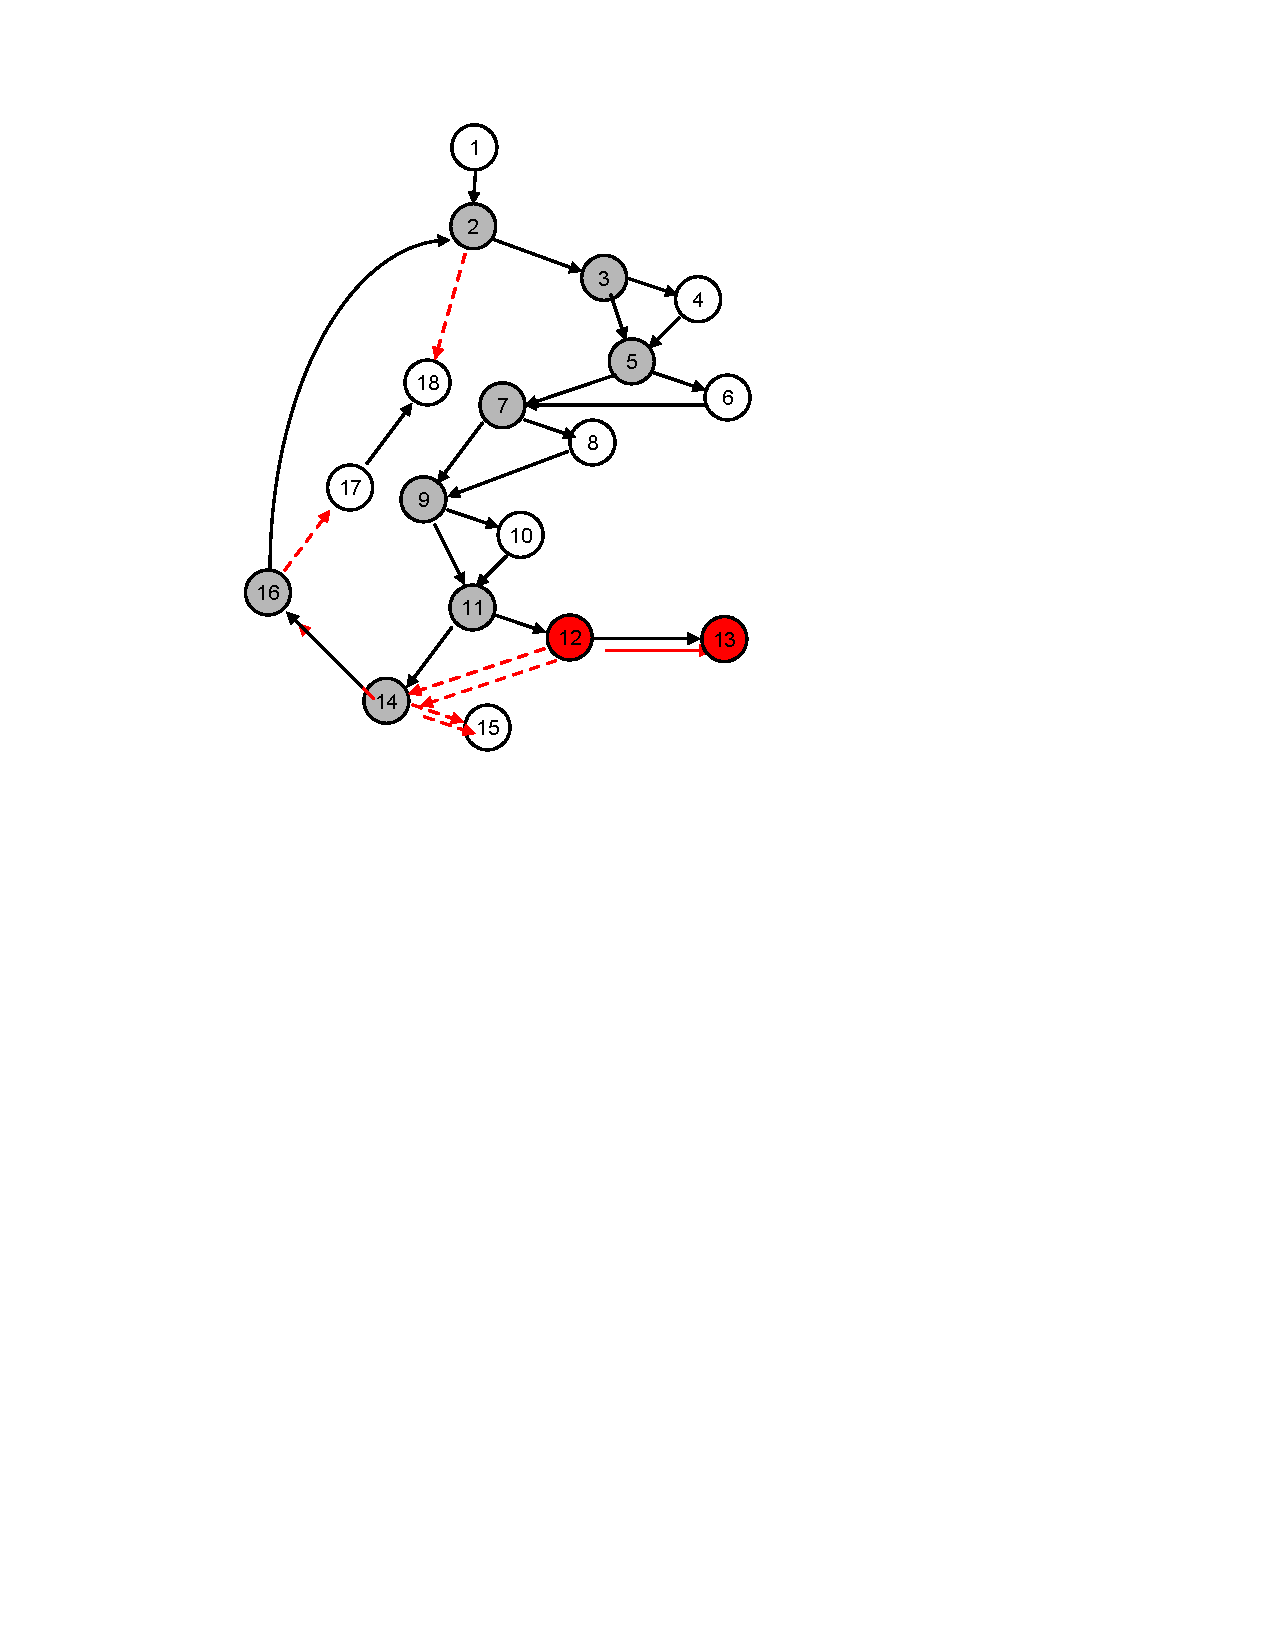
\includegraphics[width=4.5cm, keepaspectratio]{Figures/cfg}}
         \hspace{2cm}
         \subfigure{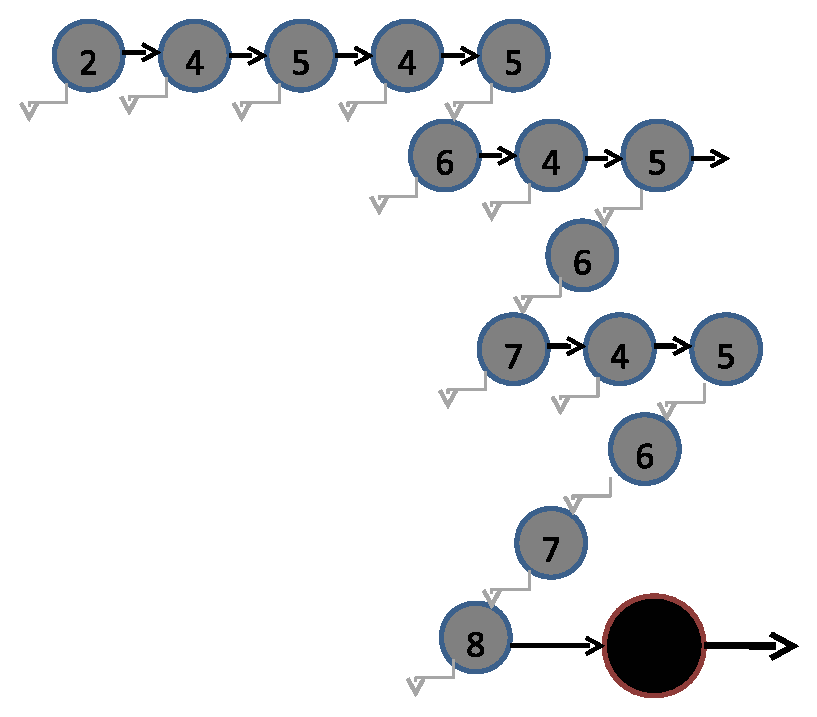
\includegraphics[width=4.5cm, keepaspectratio]{Figures/ExecutionTreeEPS}}
    \vspace{-0.4cm}
    \caption{\scriptsize{The left side of the figure shows the part of execution tree of the program for c = \{"[", "\{", "$<$", "*" \}, while the right side shows the Control-Flow Graph for the program in Figure~\ref{fig:example}.}}
    \vspace{-0.8cm}
    \label{fig:Tree}
    \end{figure}
%    \begin{figure}[t]
%    \centering
%        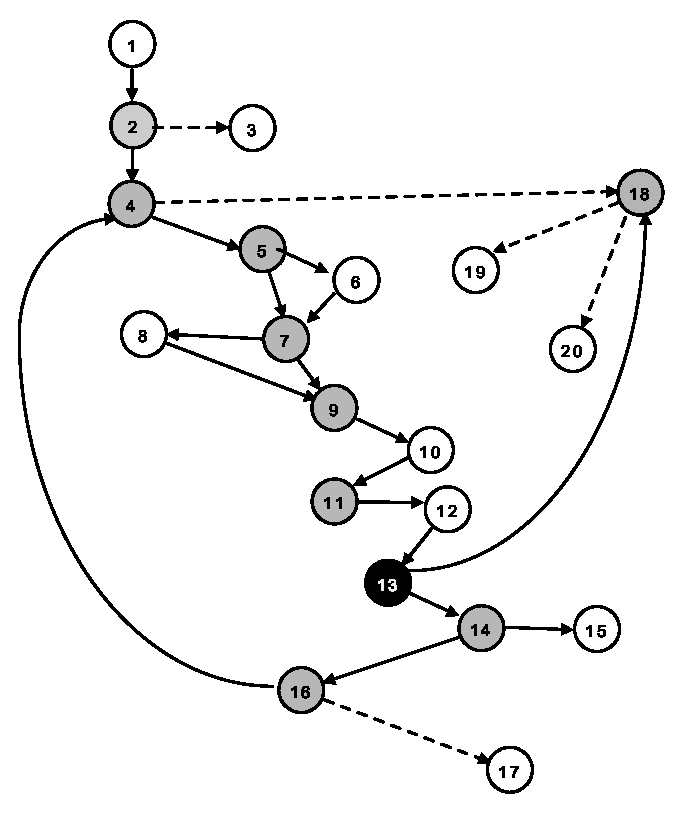
\includegraphics[width=4cm, keepaspectratio]{Figures/cfg3}
%        %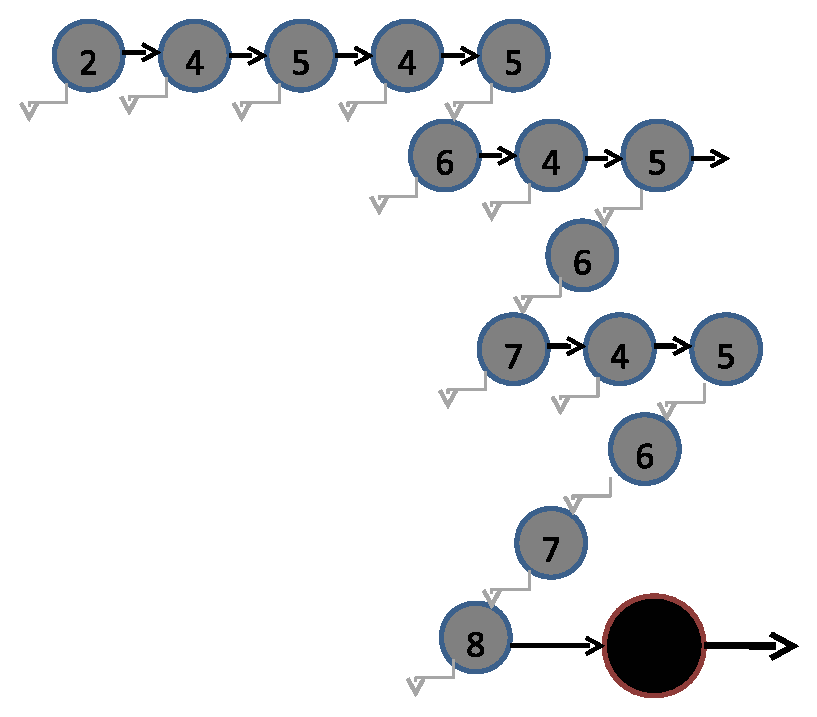
\includegraphics[width=4cm, keepaspectratio]{Figures/ExecutionTreeEPS}
%    \vspace{-0.2cm}
%    \caption{The Control-Flow Graph for the program in Figure~\ref{fig:example}}
%    \vspace{-0.5cm}
%    \label{fig:CFG}    
%	  \end{figure}
\Comment{
\\ \textbf{Instrumenter. }The Instrumenter component transforms the two versions of the
program code such that the transformed program code is
amenable to regression testing. In particular, the Instrumenter component
instruments both versions of the program under test so that program states can be compared (to determine state infection) after the execution of the added  statements at Lines 12 and 13.
}
\Comment{
	Figure~\ref{fig:Changed} shows the code of \CodeIn{testMe}'s new version after instrumentation. The \CodeIn{Instrumenter} component inserts a statement (Line 12 or 13 in Figure~\ref{fig:Changed}) just after any changed statement (Line 11 in Figure~\ref{fig:example}). The instrumented statement allows us to store the current value of \CodeIn{x} in a particular run (i.e., an explored path) of DSE. In particular, this statement results in an assertion \CodeIn{PexAssert.IsTrue ("uniqueName", x == currentX)}\footnote{\CodeIn{PexAssert} is an API class provided by Pex.} in the generated test, where \CodeIn{currentX} is the value of $x$ at Line 12 in the new version of the program. One such assertion is generated by Pex each time the statement is executed in the loop. Hence, if the loop containing the changed statement executes 20 times, 20 such assertions will be added to the test generated by Pex.
The generated test can be executed on the original version of \CodeIn{testMe} to compare program states at Line 12 after the execution of the changed statement with the ones captured in the execution of the new version. 			
\begin{figure}[t]
\begin{CodeOut}
\begin{alltt}
  \hspace{0.5cm}\textbf{public boolean} testMe(\textbf{int }x, \textbf{int[] } y)\{
  \hspace{1.0cm} ...
10\hspace{1.0cm} \textbf{if}(x == 110)\{	 
11\hspace{1.5cm} x = 2*j+1;
12\hspace{1.5cm} \textbf{PexStore.ValueForValidation}("uniqueName", x);
13\hspace{1.0cm} \} 
  \hspace{1.0cm} ...
  \}
\end{alltt}
\end{CodeOut}
\caption{Instrumented example program after instrumentation}
\label{fig:Changed}
\end{figure}
If there are multiple changed statements in the program, our approach first finds multiple regions each of which contains nearby changed statements in the program. We refer to each of such regions as a changed region in the rest of the paper. Our approach finds all the variables and fields that are identified as defined in a changed region and inserts statements (such as the statement at Line 12 of Figure \ref{fig:Changed}) to log the value of each defined variable or field in the changed region. If a defined variable is a non-primitive type, such a statement enables to compare the object graphs reachable from the logged values to compare program states. The \CodeIn{Dynamic Test Generator} component of \CodeIn{eXpress} then performs DSE on the instrumented new version of the program to generate regression tests. 
}
\Comment{
\CodeIn{eXpress} performs DSE on the instrumented new version of the program. After each run of DSE, \CodeIn{eXpress} executes the generated test on the instrumented original version (in the same way as instrumentation of the new version) to check whether the program state is infected after the execution of a changed region. The instrumentation enables us to perform only one instance of DSE on the new version instead of performing two instances of DSE: one on the original and the other on the new program version. Performing two instances of DSE can be technically challenging since we have to perform the two DSE instances in a controlled manner such that both versions are executed  with the same input and the execution trace is monitored for both the versions by a common exploration strategy to decide which branching node to flip next in the two versions. 

The Dynamic Test Generator component of \CodeIn{eXpress} uses Dynamic Symbolic Execution (DSE) to generate tests for the new version. DSE iteratively generates test inputs to cover various feasible paths in the program under test. In particular, DSE flips some branching node from a previous execution to generate a test input for covering a new path. The node to be flipped is decided by a search strategy (also called exploration starategy) such as depth-first search. Dynamic Test Generator implements a search strategy for Pex~\cite{Pex} to efficiently find behavioral differences between two versions of a program.
}
\\ \textbf{Test Generation. }To cover the changed statements at 
Lines 10 and 11 (in the left part of Figure~\ref{fig:example}) and infect the program state, 
 DSE needs at least 6 DSE runs (starting from an empty input array $c$). 
 However, the number of runs depends on the choice of branches that DSE flips in each run. 
 In each run, DSE has the choice of flipping 8 branches in the program. 
 For \CodeIn{TestMe}, Pex takes 441 DSE runs to cover the true branch of statement at Line 10. The number of runs can be much more if the number of branching statements in the program increases. To reduce the search space of DSE, \CodeIn{eXpress} prunes branches in category 
 $B_{E+I}$ until the black vertex is executed and the program state is infected after its execution.
 Once the program state is infected, \CodeIn{eXpress} prunes out the branches in category $B_{P}$ to efficiently propagate the state infection to an observable output.
\\ \textbf{Incremental Exploration.} \CodeIn{eXpress} can reuse an existing
test suite for the original version so that changed parts of the program can be explored
efficiently due to which test generation is likely to find behavior
differences earlier in path exploration. Assume that there is an existing test suite covering all the statements in the old version of the program in Figure~\ref{fig:example}. Suppose that the test suite has a test input $I$ = \{"[", "\{", "$<$", "*" \}. The input covers all the statements in the new version of \CodeIn{TestMe} except the newly added statement at Line 11. If we start the program exploration from a scratch (i.e., with default inputs), Pex takes 441 runs to cover the statement at Line 11. However, we can reuse the existing test suite for exploration to cover the new statement efficiently. Our approach executes the test suite to build an execution tree for the tests in the test suite. Our approach then starts program exploration using the dynamic execution tree built by executing the existing test suite instead of starting from an empty tree. Some branches in the tree may take many runs for Pex to discover if starting from an empty tree. Figure~\ref{fig:Tree} shows part of the execution tree for the input $I$. A gray edge in the tree indicates the false side of a branching node while a black (horizontal) edge indicates the true side. To generate an input for the next DSE runs, Pex flips a branching node $b$ in the tree whose other side has not yet been explored and generates an input so that program execution takes the unexplored branch of $b$. Pex chooses such branching node for flipping using various heuristics for covering changed regions of the program. It is likely that Pex chooses the branching node 13 (colored black), which on execution covers the \CodeIn{break} statement at Line 13. When starting the program exploration from scratch, Pex takes 420 runs before it reaches (discovers) the black branching node in Figure~\ref{fig:Tree}. Using our approach of seeding the tests from the existing test suite, Pex takes 39 runs to flip the branching node and cover the statement at Line 11.


\Comment{
\item \textbf{Branches not satisfying P}. Suppose the changed statement is executed, the program
state is infected after the execution of the changed statement, but the infection
does not propagate to an observable output.  We do
not explore the branches after the execution of the changed statement if these
branches do not lead to any other changed region.
}

\Comment{
For the example in Figure~\ref{fig:example}, our approach takes ** DSE runs to execute the changed statement, while the default strategy in Pex~\cite{Pex} takes ** DSE runs. To infect the program state, our approach takes ** DSE runs. The program state was propagated as soon as it was infected.
		}






\Comment{
\begin{figure}[t]
\begin{CodeOut}
\begin{alltt}
  [PexFactoryClass]
  \textbf{public class} FactoryClass\{
  \hspace{0.5cm}[PexFactoryMethod(typeof(\textbf{TestClassSynthesized}))]
  \hspace{0.5cm}\textbf{public static TestClassSynthesized} create(int a, 
  \hspace{1.5cm}int b, int c, int n)\{
  \hspace{1.0cm}\textbf{TestClassSynthesized} obj = 
  \hspace{1.5cm}\textbf{new} TestClassSynthesized(); 
  \hspace{1.0cm} \textbf{for}(int i=0; i< methodSeuenceLength; i++)\{
  \hspace{1.5cm} \textbf{switch}(n)
  \hspace{2.0cm} \textbf{case} 0: \textbf{obj}.A(a);\textbf{break};
  \hspace{2.0cm} \textbf{case} 1: \textbf{obj}.B(b);\textbf{break};
  \hspace{2.0cm} \textbf{case} 2: \textbf{obj}.C(c);\textbf{break};
  \hspace{2.0cm} \textbf{case} 3: \textbf{obj}.testMe();\textbf{break};
  \hspace{2.0cm} \textbf{default}: \textbf{break};
  \hspace{1.0cm}\}
  \hspace{1.5cm} \textbf{return} obj;
  \hspace{0.5cm}\}
  \}
\end{alltt}
\end{CodeOut}
\caption{Factory Class to generate an object of \CodeIn{TestClassSynthesized}}
\label{fig:factory}
\end{figure}
}




\Comment{
In this section, we illustrate our approach with the aid of an example. Our approach takes as input two versions of a class and produces as output a regression test suite. The test suite on execution detects behavioral differences between the two versions of class under test. Our approach is inspired by the PIE model~\cite{voas} of error propagation. According to the PIE model, a fault can be detected by a test suite if the fault is executed (E), the execution of the fault infects the state (I), and that the infected state propagates to the output (P). We have implemented our approach in Pex~\cite{Pex}, an automated structural testing tool based on for .NET developed at Microsoft Research. Pex uses Dynamic Symbolic Execution (DSE)~\cite{dart, cute} to explore various paths in the program and generate a unique test for each feasible path explored. To make the DSE efficiently in finding behavioral differences, our approach guides the DSE to avoid exploring irrelevant paths that cannot help in achieving E, I, or P of the PIE model.

\begin{figure}[t]
\begin{CodeOut}
\begin{alltt}
  \textbf{public} TestClass\{
  \hspace{0.5cm}\textbf{public boolean} testMe(\textbf{int }x, \textbf{int[] } y)\{
1 \hspace{1.0cm} \textbf{int} j=0, k=0;
2 \hspace{1.0cm} \textbf{if}(x==90)\{
3 \hspace{1.5cm} \textbf{for}(\textbf{int} i=0; i< y.Length; i++)\{
4 \hspace{2.0cm} \textbf{if}(y[i] == 15)
5 \hspace{2.5cm} x++;
6 \hspace{2.0cm} \textbf{else if}(y[i] == 25)
7 \hspace{2.5cm} \textbf{return} x;
8 \hspace{2.0cm} \textbf{if}(x >= 110 && x<= 150)
9 \hspace{2.5cm} j =1;
10\hspace{2.0cm} \textbf{else if}(x>150)
11\hspace{2.5cm} j =2;
12\hspace{2.0cm} \textbf{for}(i=200; i<= x; i++)
13\hspace{2.5cm} k++;
14\hspace{2.0cm} \textbf{if}(j > 0) // \textbf{if}(j >= 0)
15\hspace{2.5cm} x = j+2; //x = 2*j+1
16\hspace{2.0cm} \textbf{for}(int i=0; i< k+1; i++) 
17\hspace{2.5cm} x = x*k;
18\hspace{1.5cm} \}
19\hspace{1.0cm} \}
20\hspace{1.0cm} \textbf{return} x;
  \hspace{0.5cm}\}
  \hspace{0.5cm}...
  \hspace{0.5cm}A (\textbf{a})...
  \hspace{0.5cm}B (\textbf{b})...
  \hspace{0.5cm}C (\textbf{c})...
  \}  
\end{alltt}
\end{CodeOut}
\vspace{-0.15 in}
\caption{An Example Program}
\label{fig:example}
\end{figure}


Consider the example in Figure~\ref{fig:example}. Figure~\ref{fig:example} contains a class \CodeIn{TestClass}. The class \CodeIn{TestClass} contains a method \CodeIn{testMe} that has been changed in the new version. The class also contains 3 other methods \CodeIn{A}, \CodeIn{B}, and \CodeIn{C} that have not been changed in the new version. Suppose the statement at Line 15 of the method \CodeIn{testMe} has been modified to the one shown in the comment at Line 15. Our approach first constructs the control flow graph for the two versions and finds differences between the two control flow graphs. Our approach detects that Line 14 in the program has been changed. Instead of performing DSE separately for each version, our approach synthesizes a new class combining the two program versions as shown in Figure~\ref{fig:Changed}. As shown in Figure~\ref{fig:Changed}, our approach inserts an argument \CodeIn{isOriginalVersion} of type \CodeIn{boolean} in the method containing the changed statement. Our approach also inserts new branches at the location of changed statement(s). The \CodeIn{true} branch contains the original statement while the \CodeIn{false} branch contains the modified statement. The \CodeIn{true} branch is executed when \CodeIn{isOriginalVersion} is \CodeIn{true} and vice versa. The Line 15 in Figure~\ref{fig:example} has been changed to Lines 15-18 in Figure~\ref{fig:Changed}. The \CodeIn{true} branch of the \CodeIn{if} statement contains the original statement, while the false branch contains the statement in new version. The synthesized class \CodeIn{TestClassSynthesized} helps us in concurrently running the two versions without having to execute two instances of DSE on the two versions. After every run of DSE, we flip the \CodeIn{if(isOriginalVersion)} branch (if the branch is executed in that particular run) to check the program behavior in the new version. In the rest of this section we will refer to the program in Figure~\ref{fig:example}. Whenever we refer to comparison of program states after execution of the two versions under test, it means we flip the branch at Line 14 to execute the statement in the other version and compare the program states before and after flipping the branch. 

\begin{figure}[t]
\begin{CodeOut}
\begin{alltt}
  \textbf{public} TestClassSynthesized\{
  \hspace{0.5cm}\textbf{public boolean} testMe(\textbf{int }x, \textbf{int[] } y, 
  \hspace{3cm}\textbf{boolean} isOriginalVersion)\{
  \hspace{2.0cm} ...
14\hspace{2.0cm} \textbf{if}(j > 0)
15\hspace{2.5cm} \textbf{if}(isOriginalVersion)	 
16\hspace{3.0cm} x = j+2;
17\hspace{2.5cm} \textbf{else}
18\hspace{3.0cm} x = 2*j+1
  \hspace{2.0cm} ...
  \}
\end{alltt}
\end{CodeOut}
\vspace{-0.15 in}
\caption{Program synthesized for the example program}
\label{fig:Changed}
\end{figure}

Figure~\ref{fig:PUT} shows a Parameterized Unit Test for pex to generate tests for the method \CodeIn{testMe} in the class \CodeIn{TestClassSynthesized}. Figure~\ref{fig:factory} shows the factory method used for synthesizing an object for \CodeIn{TestClassSynthesized}. The factory method instantiates a new instance of the class \CodeIn{TestClassSynthesized}, generates a sequence of method calls containing all combinations \CodeIn{A}, \CodeIn{B}, \CodeIn{C}, and testMe. The length of the sequence is \CodeIn{methodSeuenceLength} which is set to total number of methods in the class \CodeIn{TestClassSynthesized} (4). 



\begin{figure}[t]
\begin{CodeOut}
\begin{alltt}
  [TestClass]
  \textbf{public class} PUTClass\{
  \hspace{0.5cm}[PexMethod]
  \hspace{0.5cm}\textbf{public boolean} testMePUT(\textbf{TestClassSynthesized} obj, int x, 
  \hspace{1.5cm}int[] y, boolean version)\{
 1\hspace{1.0cm}PexAssume.IsNotNull(obj);
 2\hspace{1.0cm}obj.testMe(x, y, version);
  \hspace{0.5cm}\}
  \}
\end{alltt}
\end{CodeOut}
\vspace{-0.15 in}
\caption{Parameterized test for Method \CodeIn{textMe}}
\label{fig:PUT}
\end{figure}

\begin{figure}[t]
\begin{CodeOut}
\begin{alltt}
  [PexFactoryClass]
  \textbf{public class} FactoryClass\{
  \hspace{0.5cm}[PexFactoryMethod(typeof(\textbf{TestClassSynthesized}))]
  \hspace{0.5cm}\textbf{public static TestClassSynthesized} create(int a, 
  \hspace{1.5cm}int b, int c, int n)\{
  \hspace{1.0cm}\textbf{TestClassSynthesized} obj = 
  \hspace{1.5cm}\textbf{new} TestClassSynthesized(); 
  \hspace{1.0cm} \textbf{for}(int i=0; i< methodSeuenceLength; i++)\{
  \hspace{1.5cm} \textbf{switch}(n)
  \hspace{2.0cm} \textbf{case} 0: \textbf{obj}.A(a);\textbf{break};
  \hspace{2.0cm} \textbf{case} 1: \textbf{obj}.B(b);\textbf{break};
  \hspace{2.0cm} \textbf{case} 2: \textbf{obj}.C(c);\textbf{break};
  \hspace{2.0cm} \textbf{case} 3: \textbf{obj}.testMe();\textbf{break};
  \hspace{2.0cm} \textbf{default}: \textbf{break};
  \hspace{1.0cm}\}
  \hspace{1.5cm} \textbf{return} obj;
  \hspace{0.5cm}\}
  \}
\end{alltt}
\end{CodeOut}
\vspace{-0.15 in}
\caption{Factory Class to generate an object of \CodeIn{TestClassSynthesized}}
\label{fig:factory}
\end{figure}

Our approach works in three phases (1) The Execution Phase (2) The Infection Phase (3) The Propagation Phase . 
\\ \textbf{Execution Phase.} In the Execution Phase, our approach guides the DSE in Pex to execute the changed statement(s) (at Line 15 of Figure~\ref{fig:example}). Our approach first finds all the branches that do not need to be explored for executing the changed statement at Line 15 (of Figure~\ref{fig:example}).  Our approach finds that the branches 6 and 16 (of Figure~\ref{fig:example}) cannot lead to the execution of statement at Line 15 (of Figure~\ref{fig:example}). Hence, our approach prevents Pex from exploring these branch in Execution Phase. 
 
\textbf{Infection Phase. }  The execution of the changed statement does not guarantee the infection of the program state. We compare the program state after the execution of the changed statement in the old and new version of the program under test to detect if the program state is infected. If the program state is not infected after the execution of a changed statement, our approach prevents Pex from exploring the branches after the execution of changed statement. For example, in Figure~\ref{fig:example}, the loop at Line 16 is not explored. 

\textbf{Propagation Phase. } The infected program state does not guarantee that the infection will be propagated to an observation point. We consider the last statement executed in a method as an observation point. All the \CodeIn{return} statements are considered as observation points. If a method does not has any return statement, the observation point is the last statement executed in the program. In this phase, we try to propagate the infection to one observation point at a time.
The method \CodeIn{testMe} in Figure~\ref{fig:example} has 2 observation point at Lines 7 and 20. Since the changed statement is not reachable to he observation point at Line 7, we only consider observation point at Line 20. The program state at an observation point consists of return value and the object fields. We check whether the infected state at Line 15 for the input $I_{63}$ is propagated to the end of program. This is done by comparing the return values and the value of fields after the execution of the return statement at Line 20. Our approach detects that the return value at Line 20 is the same for both versions. Our approach finds the propagation stopping statement by comparing the states after execution of all the statements executed between the changed statement at Line 15 and the return statement at Line 20. Our approach finds that the propagation is stopped after the execution of statement at line 17. The statement at line 17 is now the point of interest. The branches are prioritized based on the data dependence from statement at Line 17. Branches 12 is given the priority score $p=1$, Branch 4 is assigned a priority of score $p=2$, while branch 3 is assigned a score $p=3$. Branch 12 cannot be flipped due to infeasible path condition, hence branch 4 is flipped. The preceding process is continued 50 times until an input is generated that executes the path $P_{113}= 2T, (3T, 4T, 6F, 8F, 10F, 12F, 14F, 16F)^{110},$ $3T, 4T, 6F, 8F, 10T, 12T, 12F, 14T, 16F, 3F$, which results in the propagation of the program infection.
}
  

%\section{Problem Definition}

In this section, we present formal definitions of terms that we use throughout this paper.
In addition, we formally define the regression test generation problem that 
we address in this paper. 

We use concrete-state representation from our previous work~\cite{xie04:rostra} 
to represent the state of an object. The formal definitions of 
 Object State and Object State Equivalence  can be found 
in our previous work~\cite{xie04:rostra}. 

\Comment{
We also call each part a \Intro{heap}
and view it as a graph: nodes represent objects, and edges represent
fields. Let $P$ be the set consisting of all primitive values,
including \CodeIn{null}, integers, etc. Let $O$ be a set of objects
whose fields form a set $F$. (Each object has a field that
represents its class, and array elements are considered
index-labeled fields of the array objects.)
\define{Heap.}
{
%When a variable (such as the return or receiver of a method
%invocation) is a non-primitive-type object, we use concrete-state
%representation from our previous work~\cite{xie04:rostra} to
%represent the variable's value or state. 
%A program executes on the
%program state that includes a program heap. 
%The concrete-state representation of an object considers only parts of the heap that
%are reachable from the object. 
%We also call each part a \Intro{heap}
%and view it as a graph: nodes represent objects, and edges represent
%fields. Let $P$ be the set consisting of all primitive values,
%including \CodeIn{null}, integers, etc. Let $O$ be a set of objects
%whose fields form a set $F$. (Each object has a field that
%represents its class, and array elements are considered
%index-labelled fields of the array objects.)\\\\
A \emph{heap} is an edge-labeled graph $\Pair{O}{E}$, where
$E=\SetSuch{\Triple{o}{f}{o'}}{o \in O, f \in F, o' \in O \cup
P}$.
}
Heap isomorphism is defined as graph isomorphism based on node
bijection~\cite{boyapata02-korat}.
%\vspace*{-0.5ex}
\define{Heap Isomorphism.}{
Two heaps $\Pair{O_1}{E_1}$ and $\Pair{O_2}{E_2}$ are
\emph{isomorphic} iff there is a bijection $\rho: O_1 \to O_2$
such that:
\begin{eqnarray}
E_2 & = & \SetSuch{\Triple{\rho(o)}{f}{\rho(o')}}{\Triple{o}{f}{o'} \in E_1, o' \in O_1} \cup \nonumber\\
    &   & \SetSuch{\Triple{\rho(o)}{f}{o'}}{\Triple{o}{f}{o'} \in E_1, o' \in P}. \nonumber
\end{eqnarray}
}
%\vspace*{-1ex}
 The definition allows only object identities to vary:
two isomorphic heaps have the same fields for all objects and the
same values for all primitive fields.
\define{Object State.}
{
The state of an object $r$ is represented with a \emph{rooted} heap:
%\vspace*{-0.5ex}
A \emph{rooted heap} is a pair $\Pair{r}{h}$ of the root object $r$ and a
heap $h$ whose all nodes are reachable from $r$.
}

\define{Object State Equivalence.}
{
Two object states $s_1=\Pair{r_1}{h_1}$ and $s_2=\Pair{r_2}{h_2}$ are equivalent ($s_1 \equiv s_2$)
iff heap $h_1$ is isomorphic with heap $h_2$.
}
}

\vspace{-0.3cm}
\define {Program Execution Point.}{
Let $S= ( s_1, s_2,...,s_n)$ be the sequence of statements executed during a 
program execution $V(I)$ (i.e., when program $V$ is executed with a list of argument values $I$). 
Since a statement $s$ can be executed multiple times, multiple instances of $s$ 
can be present in $S$. A program execution point (in short an execution point) for a program execution $V(I)$
is a statement $s_i \in S$ such that statements $(s_1, s_2..., s_{i})$ have already been executed
but statements $s_{i+1}, s_{i+1},.. s_{n}$ are yet to be executed.
}
\vspace{-0.6cm}
\define{Program State.}
{
Let $M = \{m_1, m_2, m_3,..., m_n\}$ be the set of methods in 
the program call stack at an execution point $e$. 
Let $R = \{o_1, o_2, o_3,..., o_l\}$ be the set of objects such that $o_i$ is the 
receiver object of $m_i$, $A = \{ a_1, a_2,..., a_m\}$ be the set of all the arguments 
(primitive or non primitive) to methods in $M$, and 
$L= \{l_1, l_2, l_3,..., l_x\}$ be the set of all the in-scope local and global variables (primitive or non-primitive) 
at the statements  
$P = \{p_1, p_2, p_3,..., p_y, s_e\}$, where $p_i$ is the statement at which method $m_i$ is invoked and the 
$s_e$ is the statement corresponding to the execution point $e$.
The program state at an execution point $e$ is the set of object states $S_R \cup S_A \cup S_L$, where 
 $S_R = \{S_{o1}, S_{o2}, S_{o3}..., S_{ol}\}$ ($S_{oi}$
is the object state for object $o_i$ at $e$), 
 $S_A = \{S_{a1}, S_{a2}, S_{a3}..., S_{an}\}$ 
($S_{ai}$ is the object state for $a_i$ if $a_i$ is non-primitive otherwise 
$S_{ai}$ is the value of $a_i$), and $S_L = \{S_{l1}, S_{l2}, S_{l3}..., S_{lx}\}$ 
($S_{li}$ is the object state for $l_i$ at $s_e$ if $l_i$ is non-primitive otherwise 
$S_{li}$ is the value of $l_i$). 
}

%An object oriented program $P$ consists of a set 
%of classes $C = \{c_1, c_2, ..., c_l\}$. Each class $c_i$ contains a set of methods 
%$M_i = \{m_{i1}, m_{i2},..., m_{im}\}$ and a set of fields $F_i = \{f_{i1}, f_{i2},..., f_{in}\}$. 
%A method $m$ takes a set of arguments $I= \{i_1, i_2,...,\ i_o\}$ and the receiver object state $S_{R0}$ and produces as output $\Omega$ and a resulting receiver object state $S_{R1}$.
%An input $i \in I$ can be of a primitive type 

\Comment{
\define{Object State.}
{
State $S_o$ of an object $O$ (instantiated from class $C$) at a point $p$ in 
method $M$ in class $C$ is
defined by the values of fields $F$ in $C$ and the set of in-scope local variables $L$ at point $p$.
%\begin{center}
\\ \\
$S_o = \{<V(f_1), V(f_2),..., V(f_n), V(l_1), V(l_2), ..., V(l_m)>|f_i\in F,$ $V(x)$ is the 
value of $x,$ $l_i\in L\}$ 
%\end{center}
 \\ \\ 
Two program states $S_{o1}$ and $S_{o2}$ of the object $O$ at point $p$  
are equivalent ($S_{o1} \equiv S_{o2}$) if all fields 
$f_{i}\in F$ and all in-scope variables $L_j \in L$ 
of Program $P$ have equal values\footnote{
If a field $f_i$ (or an in-scope variable $l_i$) is of non-primitive type $V_1(f_i)$ (or $V_1(l_i)$) should be a deep clone of $V_2(f_i)$ (or $V_2(l_i)$).}
, i.e., $V_1(f_i) = V_2(f_i)$ (and $V_1(l_i) = V_2(l_i)$), 
where $V_1(x)$ is the value of field (or variable) x in $S_{o1}$ and 
$V_2(x)$ is the value of field (or variable) x in $S_{o2}$. 
%\footnote{Value of a non primitive type field is define by graph}.   
}

\define{Program State.}
{
Let $M = \{m_1, m_2, m_3,..., m_n\}$ be the set of methods in 
the program call stack at an execution point $e$. 
Let $R = \{o_1, o_2, o_3,..., o_n\}$ be the set of objects such that $o_i$ is the 
receiver object of $m_i$. 
Program state at an execution point $e$ is the set of object states of 
all the receiver objects $S_P = \{S_{o1}, S_{o2}, S_{o3}..., S_{on}\}$, where $S_{oi}$
is the object state for object $o_i$ at point of invocation of method $m_i$.  
}
}
\vspace{-0.2cm}
Let a program version $V$ be modified to incorporate a set of changes 
$\Delta$.
We assume that signatures of methods in $V$ are not changed and no new fields are added, modified, or deleted in $V$. 
$\Delta$ also includes the new statements added to $V$ and statements deleted from $V$.
The program version $V'$ is the resulting program version after   
$\Delta$ is applied to the program version $V$. A method $M$ in $V$
corresponds to a method $M'$ (denoted as $M \leftrightarrow M'$) in $V'$ if $M$ and $M'$ have the same signatures.
Assume that some dummy statements
are added to 
the two program versions for matching added/deleted statements between the two versions (as done by Santelices et al.~\cite{santelices}). 
These dummy statements make sure that 
a statement $s$ in $V$ can be mapped to a corresponding statement $s'$ in $V'$. 

\define{Execution Index~\cite{xin-pldi08}.}
{
An execution Index $E_{V(I)}$ of a program execution $V(I)$ is the function of execution points in 
$V(I)$ that satisfies the following property:
for any two execution points $x \in V(I)$ and $y \in V(I)$ $:$ if $x \neq y \Rightarrow E_{V(I)}(x) \neq E_{V(I)}(y) $
}
\vspace{-0.3cm}
\define{Corresponding Execution Points~\cite{xin-pldi08}.}
{
An execution point $e$ in the execution $V(I)$ corresponds to an
execution point $e'$ (denoted as $e \leftrightarrow e'$) in the execution $V'(I)$ 
($V'$ is a modified version of $V$) when $E_{V(I)}(e) = E_{V'(I)}(e')$.
For an execution point $e$ in the execution $V(I)$, there may or may not be a
corresponding execution point $e'$ in the execution $V'(I)$.
}
\vspace{-0.3cm}
\define{Parameterized Unit Test (PUT).}
{
In our formal model, we assume that a program is invoked through a 
Parametrized Unit Test (PUT)~\cite{tillmann05:parameterized}. 
A PUT $P_V =  <A, S, \lambda> $ is a method with a list of arguments $A$
and a list of statements $S=(s_1, s_2, ..s_n)$
such that $s_i \in S$ is a statement other than an assertion statement and $\lambda$ is a list of assertion statements. 
}
\vspace{-0.3cm}
\define{Corresponding PUTs.}
{
In our formal model, we assume that a program is invoked through a 
Parametrized Unit Test (PUT)~\cite{tillmann05:parameterized}. 
A PUT $P_V = <A, S, \lambda>$ in a program version $V$, corresponds to a PUT $P_{V'} = <A', S', \lambda'>$ (denoted as $P_V \leftrightarrow P_V'$), in program version $V'$ if
$V$ and $V'$ are different versions of a same program, $A = A'$, $S = S'$, and $\lambda = \lambda'$.
}


%\define{Parameterized Unit Test (PUT).}
%{
%In our formal model, we assume that a program is invoked through a 
%Parametrized Unit Test (PUT)~\cite{tillmann05:parameterized}. 
%A PUT $P_V = <V, I, M, \lambda> $ takes as input a list of arguments $A =(a_1, a_2,..., a_k)$, where $a_i$
%is a primitive or a non-primitive argument. 
%$P_V$ invokes the list of methods $M = (m_1, m_2, m_3,..., m_n)$ 
%in program version $V$  
%%with list of arguments $I_M = (I_1, I_2, I_3,..., I_n)$ such that if $i\in I_i \Rightarrow i \in I$ 
%and 
%asserts the behavior of $V$ using a list of assertions $\lambda$. We consider $I$ as inputs to the program version $V$.
%}
%\vspace{-0.5cm}
%\define{Corresponding PUTs.}
%{
%Two PUTs $P_V = <V, I, M, \lambda>$ and $P_{V'} = <V', I, M', \lambda>$ are corresponding (denoted as $P_V \leftrightarrow P_V'$) if
%$V$ and $V'$ are two versions of the same program, all the methods 
%$M = \{m_1, m_2, m_3,..., m_n\}$ invoked in $P_V$ are replaced with invocations to corresponding methods
% $M' = \{m'_1, m'_2, m'_3,..., m'_n\}$ in $V'$, respectively. 
%}
\vspace{-0.5cm}
%\define{Program State Infection.}
%{
%Two corresponding PUTs $P_V$ and $P_{V'}$ are invoked with a list of arguments (input) $I =(a_1, a_2,..., a_k)$.
%The input $I$ causes program state infection if the program state at some execution point 
%$e \in V(I)$ is $S$ and the program state at the corresponding program point
%$e' \in V'(I)$ is $S'$ such that $\neg (S \equiv S')$. If a corresponding point $e'$ does not exist,
% program state at $e \in P_V(I)$ is considered to be infected.
%}
\define{Infected Program State.}
{
The program state  of a program version $V'$ (invoked from PUT $P_{V'}$) is infected with respect to a 
program version $V$ (invoked by PUT $P_{V}$: $P_V \leftrightarrow P_V'$) 
at an execution point $e'\in V'(I)$, if 
$\exists e \in V(I): e \leftrightarrow e' $, program state of $V'$ at $e'$ is $S'$ and program state of $V$ at
$e \in V(I)$ is $S$, and $S$ is not equivalent to $S'$ (definition of equivalent states can be found in our previous work~\cite{xie04:rostra}).
}

\vspace{-0.5cm}
\define{Behavioral Difference.} 
{
Two corresponding PUTs $P_V$ and $P_{V'}$ are invoked with a list of argument values (input) $I =(a_1, a_2,..., a_k)$.
There is a behavioral difference between $V$ and $V'$ if there exists an input $I$ such that 
when $P_V$ and $P_{V'}$ are invoked with input $I$, $\exists \lambda_i \in \lambda$ such that $\lambda_i$ passes
for $P_V$ but fails for $P_V'$ or $\lambda_i$ fails
for $P_V$ but passes for $P_V'$. $I$ is referred to as an input detecting behavioral difference.
}
\vspace{-0.5cm}
\define{Problem Definition.} 
{
Regression test generation for a PUT $P_{V'}$ in program version $V'$
is the problem of generating an input $I$ for $P_{V'}$  
that detects behavioral difference 
between $V$ and $V'$.
This paper focuses on efficiently generating inputs detecting behavioral differences.
}

\section{Approach}
\label{sec:approach}

Our approach accepts a set of projects as data sources and mines
API mapping between two different languages $L_1$ and $L_2$.
As mined API mapping describes mapping relations of APIs between
the two languages, this mapping is useful for language migration between the two languages.
For each project used as a data source, our approach requires
atleast two versions of the project (one version in $L_1$ and
the other version in $L_2$). Figure~\ref{fig:approach} shows
the overview of our approach.

First, our approach aligns client code in languages $L_1$ and $L_2$
so that the aligned source files implement similar functionalities
(Section~\ref{sec:approach:acc}). Second, our approach mines
mapping relations of API classes (Section~\ref{sec:approach:mappingtypes}).
Finally, our approach mines mapping relations of API
methods (Section~\ref{sec:approach:mappingtypes}) defined by the mapped
API classes.

\begin{figure}[t]
\centering
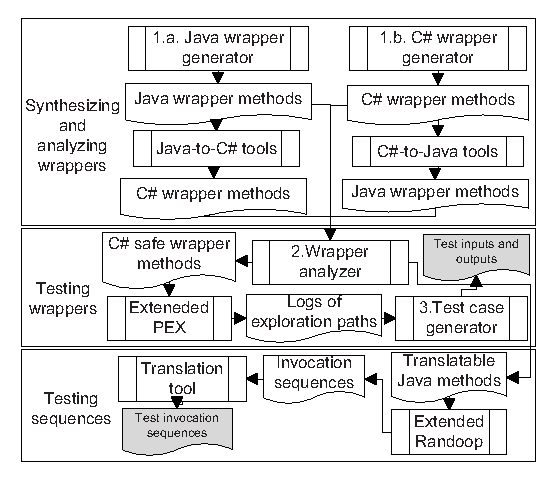
\includegraphics[scale=1,clip]{figure/approach.eps}\vspace*{-3ex}
 \caption{Overview of our approach}\vspace*{-3.5ex}
 \label{fig:approach}
\end{figure}

%-------------------------------------------------------------------
\subsection{Aligning Client Code}
\label{sec:approach:acc}

Initially, our approach accepts two versions of a project (one version in
$L_1$ and the other version in $L_2$) and aligns classes and methods
of the two versions. Aligned classes or methods
between the two versions implement a similar functionality. As they
implement a similar functionality, APIs used by these classes or methods can be
replaceable.

To align classes and methods of the two versions, our approach uses
name similarities between entities (such as class names or method names)
defined by the two versions of the project. In our approach, we have two
different kinds of entity names: entity names defined by the two versions
of the project and entity names of third-party libraries used by the two versions of the project.
The first kind often comes from the same programmer or the same team, or
programmers may refer to existing versions for naming entities such
as classes, methods, and variables. Therefore, name similarity is often
reliable to distinguish functionalities of the first kind compared to the second
kind. Our approach uses Simmetrics\footnote{\url{http://sourceforge.net/projects/simmetrics/}}
to calculate name similarities.

Algorithm 1 shows how our approach aligns client code classes. The
first step is to find candidate class pairs by names. For two sets
of classes ($C$ and $C'$), the algorithm returns candidate class
pairs ($M$) with a similarity greater than a given threshold,
referred to as \emph{SIM\_THRESHOLD}. As some projects may have many
classes with the same name, $M$ may contain more than one matching
pair for a class in a version. To align those classes, our algorithm
uses package names of these classes to refine $M$ and returns only
one matching pair with the maximum similarity\footnote{For C\#, we
refer to namespace names for package names.}.

In each aligned class pair, our approach further aligns methods
within the class pair. The algorithm for methods is similar to the
algorithm for classes but relies on other criteria such as the number of parameters
and names of parameters to refine candidate method pairs. These candidates
may contain more than one method pair due to overloading.
For the example shown in Section~\ref{sec:example}, our approach
correctly aligns the class \CodeIn{IndexFiles} and the method
\CodeIn{main} in Java to the class \CodeIn{IndexFiles}
and the method \CodeIn{Main} in C\# as their names are quite
similar.
%-----------------------------------------------------------------
\subsection{Mapping API classes}
\label{sec:approach:mappingtypes}

In this step, our approach mines mapping relations of
API classes. As defined in Section~\ref{sec:mapping}, mapping relations of API classes are used
to translate variables. Consequently, our approach mines mapping
relations of API classes based on how aligned client code declares
variables such as fields of aligned classes, parameters of aligned methods
and local variables of aligned methods. In
particular, for each aligned class pair $\Pair{c_1} {c_2}$, our
approach analyzes each field pair $\Pair{f_1}{f_2}$ and considers
$\Pair{f_1.type} {f_2.type}$ as one mined mapping relation of API
classes when the similarity between $f_1.name$ and $f_2.name$ is
greater than \emph{SIM\_THRESHOLD}. Similarly, for each aligned method pair
$\Pair{m_1} {m_2}$, our approach analyzes each local variable pair
$\Pair{var_1} {var_2}$ and considers $\langle var_1.type,$ $
var_2.type\rangle$ as one mined mapping relation of API classes when
the similarity between $var_1.name$ and $var_2.name$ is greater than
a threshold. Also, our approach analyzes each parameter pair
$\langle para_1, $ $para_2\rangle$ of $m_1$ and $m_2$, and our
approach considers $\langle para_1.type,$ $para_2.type\rangle$ as
one mined mapping relation of API classes when the similarity
between $para_1.name$ and $para_2.name$ is greater than \emph{SIM\_THRESHOLD}.

For the example shown in Section~\ref{sec:example}, our approach
mines the mapping relation between \CodeIn{java.io.File} and
\CodeIn{System.IO.FileInfo} based on the matched fields of Lines 4
and 9 (Figure~\ref{fig:clientcode}). The mapping relation of API classes helps translate the
variable declared in Line 1 (Figure~\ref{fig:totranslation})
to the variable declared in Line 16 (Figure~\ref{fig:translatedcode}).

%\begin{algorithm}[t]
%\begin{SmallOut}
%\dontprintsemicolon
%  \KwIn{$C$ is the classes of a language; $C'$ is the classes
%  of another language}
%  \KwOut{$P$ is aligned pairs of classes}
%  \Begin{
%     $M \leftarrow findCandidateClassPairs(C, C')$\;
%     \While{$M.size > 0 $}{
%        \If{$M.size > 1$}{
%            $M \leftarrow refineByPackageNames(M)$\;
%         }
%         \If{$M.size == 1$}{
%                $P.add(M)$\;
%                $C.remove(M[0].c)$\;
%                $C'.remove(M[0].c')$\;
%         }
%         $M \leftarrow findCandidateClassPairs(C, C')$\;
%     }
% }
%\end{SmallOut}
%\label{alg:alignclasses} \caption{Align Classes Algorithm}
%\end{algorithm}

\begin{figure}[t]
\centering
\includegraphics[scale=1,clip]{figure/algorithm1.eps}
\vspace*{-6ex}
\end{figure}

%-----------------------------------------------------------
\subsection{Mapping API methods}
\label{sec:approach:mappingtypes}

In this step, our approach mines mapping relations of API methods.
This step has two major sub-steps. First, our approach builds a graph, referred
as API transformation graph, for each client code
method. Second, our approach compares the two graphs of each paired
client code methods for mining mapping relations of API methods.

\begin{figure*}[t]
\centering
\includegraphics[scale=1.1,clip]{figure/graph.eps}\vspace*{-3ex}
 \caption
{\label{fig:graph}Built ATGs and the main steps of comparing
ATGs}\vspace*{-3.5ex}
\end{figure*}


\subsubsection{API transformation graph}
We propose API transformation graphs (ATG) to help deal with the two
challenges of mining API mapping listed in
Section~\ref{sec:introduction}. An API transformation graph of a
client code method $m$ is a directed graph
$G\Triple{N_{data}}{N_{m}}{E}$. $N_{data}$ is a set of the fields
$F$ of $m$'s declaring class, local variables $V$ of $m$, parameters
$P_1$ of $m$, parameters $P_2$ of methods called by $m$, and return
values $R$ of all methods. $N_{m}$ is a set of methods called by
$m$. $E$ is a set of directed edges. An edge $d_1\rightarrow d_2$
from a datum $d_1 \in N_{data}$ to a datum $d_2 \in N_{data}$
denotes the data dependency from $d_1$ to $d_2$. An edge $d_1
\rightarrow m_1$ from a datum $d_1 \in N_{data}$  to a method $ m_1
\in N_{m}$ denotes $d_1$ is a parameter or a related variable of
$m_1$. An edge $m_1 \rightarrow d_1$ from a method $m_1 \in N_{m}$
to a datum $d_1 \in N_{data}$ denotes $d_1$ is the return value of
$m_1$.

%We propose ATG for two main purposes. The first purpose is to mine mapping
%relations among parameters of mapped API methods. Mining mapping relations
%among parameters of mapped API methods is challenging as often mapped API methods
%can have different number of parameters or different positions among
%parameters. For example, consider the following two mapped API methods:
%
%\begin{CodeOut}
%$m_1$ in Java: BigDecimal java.math.BigDecimal.multiply (BigDecimal $p_1^1$)\\
%\hspace*{0.11in}$m_2$ in C\#: Decimal System.Decimal.Multiply (Decimal $p_1^2$, Decimal $p_2^2$)
%\end{CodeOut}
%
%Method $m_1$ of Java has a receiver variable, say $v_1^1$, of type \CodeIn{BigDecimal}
%and has one parameter $p_1^1$. The mapped method $m_2$ in C\# has
%two parameters $p_1^2$ and $p_2^2$. Using ATGs, our approach
%identifies that $v_1^1$ is mapped to $p_1^2$ and $p_1^1$ is mapped
%to $p_2^2$. As ATG captures parameters of API methods,
%our approach is able to deal with the challenges of mapping parameters.
%
%The second purpose of ATG is to mine mapping relations of merged API methods. As ATG
%describes data dependencies among inputs and outputs, our approach
%is able to mine mapping relations for merged API methods as shown in
%Figure~\ref{fig:example}. We next describe how our approach builds ATGs and
%uses ATGs for mining mapping relations of API methods.

\subsubsection{Building API transformation graphs }

Our approach builds an ATG for each method $m$. ATG includes information such as
inputs and outputs for each client code method. In particular, for
each method $m$, our approach first builds subgraph for its variables,
API methods, and field accesses according to the following rules:

%First, programming languages typically provide a huge set of APIs,
%and it is difficult to build mapping relations for all APIs
%manually. Second, some API methods have multiple parameters, and
%some parameters cannot be mapped directly one by one in orders. For
%example, \CodeIn{org.w3c.dom.Element.getAttributeNS()} and
%\CodeIn{System.Xml.XmlElement.GetAttribute()} both have two
%parameters, but the two parameters are inverse by their meanings.
%Third, one API method in one language may be mapped to more than one
%API method in other languages. For example, \CodeIn{java.util.
%LinkedList.removeLast()} returns the last value, and \CodeIn{System.
%Collections.Generic.LinkedList.RemoveLast()} does not return any
%values. To get that value, C\# programmers need to call more APIs,
%and thus one API method of Java is mapped to serval API methods of
%C\#.



%
%One challenge to mine mapping relations of two API methods lies in
%how to map their inputs correctly. Here, our approach both the
%receiver and the parameters of a method as the inputs of a
%method. Inputs of two API methods may be matched but are not in the
%same order. For example, as shown in Section~\ref{sec:example},
%\CodeIn{java.io. File.exist()} has a receiver whereas
%\CodeIn{System.IO.File.Exist()} has no receiver but a
%parameter. In addition, parameter orders may be quite different. For
%example, the parameter order of \CodeIn{org.w3c.
%dom.Element.getAttributeNS()} is inverse with the parameter order of
%\CodeIn{System.Xml.XmlElement.GetAttribute()}. To deal with the
%preceding problem,


\begin{enumerate}\vspace*{-2ex}
\item $\forall$ $f \in F \cup V \cup P_1$, our approach adds a node to the built ATG.
The reason for considering these variables such as fields in
declaring class or local variables in method $m$ used in client code
is that these variables are useful to analyze data dependencies
among API methods.\vspace*{-2ex}
%\begin{center}
%\includegraphics[scale=0.7,clip]{figure/rule1.eps}
%\end{center}
\item $\forall$ API methods of the form ``$T_0\ T.AM (T_1 p_1, \ldots, T_n p_n)$''
called by method $m$, our approach adds receiver (of type $T$) and
parameter nodes to the built ATG as shown below. Our approach does
not add receiver node for static API methods. \vspace*{-3ex}
\begin{center}
\includegraphics[scale=0.7,clip]{figure/rule2.eps}%\vspace*{-1.5ex}
\end{center}\vspace*{-3ex}
\item $\forall$ $f\in F \cup V$, if $f$ is a non-primitive variable
of type $T_1$ and a field $x$ of $T_1$ is accessed as $f.x$, our
approach adds nodes to the built ATG as shown below. As Java often
uses getters and setters whereas C\# often use field accesses, our
approach treats field accesses as a special type of method
calls.\vspace*{-2ex}
\begin{center}
\includegraphics[scale=0.7,clip]{figure/rule3.eps}%\vspace*{-1.5ex}
\end{center}\vspace*{-3ex}
\end{enumerate}

Our approach adds additional edges to the built ATG (and sub-graphs
inside ATG) representing data dependencies among built sub-graphs.
We use the following rules for adding additional edges to the built
ATG. \Comment{In particular, our approach analyzes source files of a
client code method statement by statement and adds edges according
to the rules as follows:} \vspace*{-1.5ex}
\begin{enumerate}
\item $\forall$ statements of the form $x = y$, where $x \in F \cup V \wedge y \in F \cup V$,
our approach adds an edge from $y$ to $x$. This edge represents that
$x$ is data dependent on $y$.\vspace*{-1.5ex}
\begin{center}
\includegraphics[scale=0.7,clip]{figure/rule4.eps}%\vspace*{-1.5ex}
\end{center}\vspace*{-1.5ex}
\item $\forall$ statements of the form $x = AM()$, where $x \in F \cup V$, our approach
adds an edge from $AM$ to $x$ if the return value of $AM$ is
assigned to $x$. This edge represents that $x$ is data dependent on
the return value of $AM$. \vspace*{-1.5ex}
\begin{center}
\includegraphics[scale=0.7,clip]{figure/rule5.eps}%\vspace*{-1.5ex}
\end{center}\vspace*{-1.5ex}
\item $\forall$ API methods $AM(x)$ called by method $m$, our approach
adds an edge from $x$ to the parameter node of $AM$. This edge
represents that the parameter of $AM$ is data dependent on
$x$.\vspace*{-1.5ex}
\begin{center}
\includegraphics[scale=0.7,clip]{figure/rule6.eps}%\vspace*{-1.5ex}
\end{center}\vspace*{-1.5ex}
\item $\forall$ statements of the form $m_2(m_1(x))$, our approach
adds an edge from the return value node of $m_1$ to the parameter
node of $m_2$ parameter node. This edge represents that the
parameter of $m_2$ is data dependent on the return value of
$m_1$.\vspace*{-1.5ex}
\begin{center}
\includegraphics[scale=0.7,clip]{figure/rule7.eps}%\vspace*{-1.5ex}
\end{center}\vspace*{-1.5ex}
\item $\forall$ statements of the form $x.m()$, our approach adds
an edge from $x$ to $m$ as $x$ is the receiver object of $m$. This
edge represents that the receiver object of $m$ is data dependent on
$x$.\vspace*{-1.5ex}
\begin{center}
\includegraphics[scale=0.7,clip]{figure/rule8.eps}%\vspace*{-1.5ex}
\end{center}\vspace*{-1.5ex}
\item $\forall$ statements of the form $ x = y\ op\ z\ op\ \ldots, op \in \{+,-,*,/\}$,
our approach adds edges from $y$, $z$, and others to $x$, as these
variables are connected by binary operations and the return value is
assigned to $x$. The edge denotes the data dependency from $y$, $z$,
and other variables to $x$. For simplicity, our approach ignores
\emph{op} info. We discuss the issue in
Section~\ref{sec:discuss}.\vspace*{-1.5ex}
\begin{center}
\includegraphics[scale=0.7,clip]{figure/rule9.eps}%\vspace*{-1.5ex}
\end{center}\vspace*{-2ex}
\end{enumerate}

For each method $m$ in the client code, our approach applies preceding
rules for each statement from the beginning to the end of $m$.
Within each statement, our approach applies these rules based on
their nesting depth in the abstract syntax tree. For example,
for the statements of the form $m_2(m_1(x))$, our approach first applies
these rules on $m_1$ and then on $m_2$.

Figures~\ref{fig:graph}a and ~\ref{fig:graph}b show partial ATGs for
C\# (\CodeIn{IndexFiles.cs}) and Java (\CodeIn{IndexFiles.java})
code examples shown in Figure~\ref{fig:clientcode}, respectively.
Figure~\ref{fig:graph} also shows corresponding line numbers of each
sub-graph. Our approach applies Rules 2 and 6 for Lines 4 and 9 (Figure~\ref{fig:clientcode})
to build corresponding sub-graphs in the ATG. For
Lines 6 and 7 (Figure~\ref{fig:clientcode}), our approach applies Rules 2 and 8 to build
corresponding sub-graphs in the ATG. For Lines 12 and 15 (Figure~\ref{fig:clientcode}),
our approach applies Rule 2, 3, and 6 to build corresponding sub-graphs.

%\begin{algorithm}[t]
%\begin{SmallOut}
%\label{alg:mapATG} \dontprintsemicolon
%  \KwIn{$G$ is the ATG of a method ($m$); $G'$ is the ATG of $m$'s mapped method.}
%  \KwOut{$S$ is a set of mapping relations for API methods}
%  \Begin{
%     $P \leftarrow findVarPairs(m, m')$\;
%     \For{Pair p in P}{
%        $SM \leftarrow G.nextMethods(p.sharp)$\;
%        $JM \leftarrow G.nextMethods(p.java)$\;
%        $\Delta S = mapping(SM, JM)$\;
%        \While{$\Delta S \neq \phi| \Delta SM \neq \phi| \Delta JM \neq \phi$}{
%            $S.addAll(\Delta S)$\;
%             \For{Method sm in SM}{
%                 \If{$sm.isMapped$}{
%                    $SM.replace(sm, sm.nextMethod())$\;
%                  }\Else{
%                    $SM.replace(sm, sm.mergeNextMethod())$\;
%                  }
%             }
%             \For{Method jm in JM}{
%                 \If{$jm.isMapped$}{
%                    $JM.replace(jm, jm.nextMethod())$\;
%                  }\Else{
%                    $JM.replace(jm, Jm.mergeNextMethod())$\;
%                  }
%             }
%             $\Delta S = mapping(SM, JM)$\;
%        }
%     }
% }
% \end{SmallOut}
%\caption{ATG Comparison Algorithm}
%\end{algorithm}

\begin{figure}[t]
\centering
\includegraphics[scale=1,clip]{figure/algorithm2.eps}
\vspace*{-6ex}
\end{figure}

%--------------------------------------------------------------------
\subsubsection{Comparing API transformation graphs}

The second sub-step compares each pair of built ATGs for mining mapping
relations of API methods. Our mapped API methods satisfy three
criteria: (1) Mapped API methods implement the same
functionality. (2) Mapping relation describes the relation
between parameters of mapped API methods. (3) Mapping relation
describes the relation between return values of
mapped API methods. The two mapped API methods in two
different languages satisfying the preceding three criteria
are replaceable in the client code. Therefore, these mapped API
methods assist for migrating client code from one language to another.

Algorithm 2 presents major steps of comparing ATGs for mining
mapping relations of API methods. Consider two methods $m$ and $m'$
of two different languages $L$ and $L'$, respectively, in the client
code. Consider that the associated ATGs of $m$ and $m'$ are compared
to mine mapping relations of API methods. First, our algorithm finds
matching variables $\in$ $F$, $V$, and $P_1$ in $m$ and $m'$. Our
algorithm maps two variables $v$ and $v'$ of methods $m$ and $m'$,
respectively, if the similarity measure on their names is greater
than \emph{SIM\_THRESHOLD}. For constants in $m$ and $m'$, our
algorithm maps those two constants, if they have exactly the same
value. Our algorithm uses these variable and constant mappings to
compute mappings between API methods that use these variables and
constants. Our algorithm uses the following criteria for mapping two
API methods $jm$ and $sm$.

\emph{Matching entities}: The first criterion is based on entities such as receiver variable
or parameters of $jm$ and $sm$ to map $jm$ and $sm$. We map $jm$ with $sm$, if
the receiver variable of API method $jm$ is mapped
to the receiver variable of $sm$, and there is a one-to-one mapping between parameters
of $jm$ and $sm$.

\emph{Matching functionalities}: The second criterion is based on functionalities of
$jm$ and $sm$. We consider that $jm$ and $sm$ implement the same functionality,
if the similarity measure between the name of $jm$ and the name of $sm$ is
greater than \emph{SIM\_THRESHOLD}.

\emph{Matching outputs:} The third criterion is based on the return values of $jm$ and $sm$.
Consider the return values of $jm$ and $sm$ as $r_1$ and $r_2$, respectively. We map $jm$
with $sm$, if the type of $r_1$ is mapped with the type of $r_2$ in mapping API classes
relationship.

Our algorithm first attempts to map first API method $jm$ in $m$
with the first API method $sm$ in $m'$. If our algorithm successfully maps $jm$ with
$sm$, our algorithm moves to the next available API methods in $m$
and $m'$ of the client code. If our algorithm does not able to map $jm$
with $sm$, our algorithm merges $sm$ and $jm$ with their next available API methods
in the corresponding ATGs, respectively, and attempts to map merged API methods.
For two merged API methods, our algorithm uses the
maximum similarity of method names between $jm$ and $sm$ as a
similarity measure for matching their functionalities.
With each iteration, $sm$ or $jm$ or the mapping relation (represented as $S$)
in the algorithm changes. Therefore, we repeat our algorithm
till $S$, $sm$, and $jm$ do not change anymore.

We next explain our algorithm using the illustrative example shown
in Figure~\ref{fig:graph}. The numbers shown in circles
represent the major steps in our algorithm for mining mapping
relations of API methods. We next explain each step in detail.

\emph{S1: mapping parameters, fields, local variables, and constants.}
Given two ATGs of each method pair $\langle m, m' \rangle$, this step maps
variables such as parameters, fields, and local variables by comparing their names
and maps constants by comparing their values. As shown in
Figure~\ref{fig:graph}, Step 1 maps two constants as both the constants
have the same value \CodeIn{index}.

\emph{S2: mapping inputs of API methods.} Step 2 mines mapping
relations of API methods using variable and constant mapping relations.
Initially, this step identifies first API methods in the two ATGs and tries to
map their parameters and receiver objects of the two API methods.
In our current example, this step maps the parameter \CodeIn{filename}
to the parameter \CodeIn{arg0} as these parameters
are of the same type and their associated constants are mapped.

\emph{S3: mapping outputs of API methods.} In contrast to Step 2
that maps parameters, Step 3 maps return values of API methods. In
this step, if our approach is not able to map return values, our
approach merges the next API method and then attempts to map return
values of merged API methods. In our current example shown in
Figure~\ref{fig:graph}, return value of
\CodeIn{System.IO.FileInfo.FileInfo()} cannot be mapped to the
return value of \CodeIn{java.io.File.File()}. Therefore, our
approach merges next API methods in the ATG till the \CodeIn{Exists}
API method, as the return values (shown as \CodeIn{Boolean}) match
only after the \CodeIn{Exists} API method. Figure~\ref{fig:graph}
shows Step 3 along with the matching return values.

\emph{S4: mapping functionalities.} After our approach maps parameters and return values,
this step further maps functionalities of those merged API
methods. Given two merged API methods with mapped parameters and return values,
this step uses the similarity measure based of their method names as a criterion
for matching their functionalities. In the preceding example, this step maps
the two merged API methods shown in Figure~\ref{fig:graph}a to the
merged API methods of the \CodeIn{java.io.File.exist()} as all three
merged API methods include the method named \CodeIn{exist}.

Our approach applies preceding steps on ATGs
(as shown in Figures~\ref{fig:graph}a and~\ref{fig:graph}b) and mines
mapping relations. An example mapping relation from the preceding ATGs is
shown in Figure~\ref{fig:example}.

%\section{Implementation}

\section{Experiments}
\label{sec:evaluation}

We conducted experiments on four programs and their 67 versions (in total) collected from three different sources. In our experiments, we try to address the following research questions:
%\begin{itemize}
\Comment{
\\ \textbf{RQ1.} How much fewer DSE runs does Pex require to execute the changed regions between the two versions of a program with the assistance of \CodeIn{eXpress}?
	\\ \textbf{RQ2.} Can \CodeIn{eXpress} more efficiently infect the program states after the execution of changed regions than without using \CodeIn{eXpress}?	
	\\ \textbf{RQ3.} Can \CodeIn{eXpress} effectively help generate tests that execute changed regions between the two versions of a program than without using \CodeIn{eXpress}?
	\\ \textbf{RQ4.} Can \CodeIn{eXpress} effectively help generate tests that infect the program states after the execution of changed regions than without using \CodeIn{eXpress}?
	\\ \textbf{RQ5.} Can \CodeIn{eXpress} effectively help generate tests that find behavioral differences than without using \CodeIn{eXpress}?
	\\ \textbf{RQ6.} Can our approach of seeding the exploration with existing unit-tests efficiently help covering the changed regions and infect program states?
}
%\\ \textbf{RQ1.} How many fewer DSE runs does Pex require to execute the changed regions between the two versions of a program with the assistance of \CodeIn{eXpress}?
%	\\ \textbf{RQ2.} How many fewer DSE runs does Pex require to infect the program states with the assistance of \CodeIn{eXpress}?
	\\ \textbf{RQ1.} How many fewer DSE runs and how much fewer amount of time does Pex require to find behavioral differences with the assistance of \CodeIn{eXpress}?
%	\\ \textbf{RQ4.} How many more tests does Pex, with the assistance of \CodeIn{eXpress}, generate that execute changed regions between the two versions of a program?
%	\\ \textbf{RQ5.} How many more tests does Pex, with the assistance of \CodeIn{eXpress}, generate that infect the program states?
%	\\ \textbf{RQ6.} How many more tests does Pex, with the assistance of \CodeIn{eXpress}, generate that find behavioral differences?
		\\ \textbf{RQ2.} How many fewer DSE runs and how much fewer amount of time does \CodeIn{eXpress} require to infect the program state using our code instrumentation technique than without using the technique?
	\\ \textbf{RQ3.} How many fewer DSE runs and how much fewer amount of time does Pex require to find behavior differences when the program exploration is seeded with the existing test suite?


		\Comment{
	\\ \textbf{RQ6.} Can the optimizations used in \CodeIn{Graph Builder} and \CodeIn{Graph Traverser} components of \CodeIn{eXpress} efficiently reduce the time to find irrelevant branches that cannot help in satisfying E of the PIE model?
	

	\item \textbf{RQ3.} Can \CodeIn{eXpress} more efficiently propagate the program state infection to some observable output?
	
	}	
%\end{itemize}

\Comment{
\begin{table*}
\begin{CodeOut}
\begin{center}
\caption {\label{table:siena_results}Experimental Results for Siena}
\begin {tabular} {|l|c|c|c|c|c|c|c|c|}
\hline
\multicolumn{4}{|c|}{}&\multicolumn{2}{|c|}{Reused}&\multicolumn{2}{|c|}{TUT 2 PUT}\\ 
\hline
MUMs&\CenterCell{Methods Implemented
} &\CenterCell{Methods Reused
}&\CenterCell{    Increase in LOC
}&\CenterCell{   Increase in Max. CC  
}&\CenterCell{  Increase in LOC
}&\CenterCell{   Increase in Max. CC
}&\CenterCell{}\\
\hline												
												

%Total&&301&214&28.9&488&944&93.4&&&&&&&\\
\hline
\end{tabular}
\end{center}
\end{CodeOut}
\end{table*}
}

\subsection{Subjects}
\label{sec:subjects}
To address the research questions, we conducted experiments on four subjects.
Table~\ref{table:subjects} shows the details about the subjects. Column 1 shows the subject name. Column 2 shows the number of classes in the subject. Column 3 shows the number of classes that are covered by tests generated in our experiments. Column 4 shows the number of versions (not including the original version) used in our experiments. Column 5 shows the number of lines of code in the subject.
\Comment{
The experimental subjects and results can be downloaded from our our project web\footnote{\url{http://ase.csc.ncsu.edu/projects/express}}. 
}

\CodeIn{replace} and \CodeIn{siena} are programs available from the Subject Infrastructure Repository (SIR)~\cite{doESE05}. \CodeIn{replace} and \CodeIn{siena} are written in $C$ and $Java$, respectively. \CodeIn{replace} is a text-processing program, while \CodeIn{siena} is an Internet-scale event notification program. We chose these two subjects (among the others available at the SIR) in our experiments we could convert these subjects into C\# using the Java 2 CSharp Translator\footnote{\url{http://sourceforge.net/projects/j2cstranslator/}}. We could not convert other subjects available at the SIR (with the exception of \CodeIn{tcas}) because of extensive use of $C$ or $Java$ library APIs in these subjects. The experimental results on \CodeIn{tcas} are presented in a previous version of this work~\cite{taneja09:guided} and show similar conclusions as the results from the subjects used in the experiments here. We seeded all the 32 faults available for \CodeIn{replace} at the SIR one by one to generate 32 new versions of \CodeIn{replace}. For \CodeIn{siena}, SIR contains 8 different sequentially released versions of \CodeIn{siena} (versions 1.8 through 1.15). Each version provides enhanced functionalities or corrections with respect to the preceding version. We use these 8 versions in our experiments. In addition to these 8 versions, there are 9 seeded faults available at SIR. We seeded all the 9 faults available at SIR one by one to synthesize 9 new versions of \CodeIn{siena}. 
In total, we conduct experiments on these 17 versions of \CodeIn{siena}. For \CodeIn{replace}, we use the \CodeIn{main} method as a PUT for generating tests. We capture the concrete value of the string $sub$ at the end of the $PUT$ using \CodeIn{PexStore.ValueForValidation("v", v)} statement. This statement captures the current value of $v$ in a particular run
(i.e., an explored path) of DSE. In particular, this statement
results in an assertion \CodeIn{Assert.AreEqual(v, cv)} in a generated test, where $cv$ is the concrete value of $v$ in the test during the time of exploration. 
This assertion is used to find behavioral differences when the tests generated for a new version are executed on the original version. For \CodeIn{siena}, we use the methods \CodeIn{encode} (for changes that are transitively reachable from \CodeIn{encode}) and \CodeIn{decode} (for changes that are transitively reachable from \CodeIn{decode}) in the class \CodeIn{SENP} as PUTs for generating tests. We capture the return values of these methods using the \CodeIn{PexStore} statement 
in the PUTs.

%The method \CodeIn{encode} requires non-primitive arguments. Existing Pex cannot handle non-primitive argument types effectively but provides support for using factory methods for non-primitive types. Hence, we manually wrote factory methods for the non-primitive types in \CodeIn{SENP}. In particular, we wrote factory methods for classes \CodeIn{SENPPacket}, \CodeIn{Event} and \CodeIn{Filter}. Each factory method invokes a sequence (of length up to three) of the public state-modifying methods in the corresponding class. The parameters for these methods, and the length of the sequence (up to three) are passed as inputs to the factory methods. During exploration, Pex generates concrete values for these inputs to cover various parts of the program under test.

STPG\footnote{\url{http://stringtopathgeometry.codeplex.com/}} and is an open source program hosted by the codeplex website. The codeplex website contains snapshots of check-ins in the code repositories for STPG. We collect three different versions of the subject STPG from the three most recent check-ins. We use the \CodeIn{Convert(string path)} method as the PUT for generating tests since \CodeIn{Convert} is the main conversion method that converts a string path data definition to a \CodeIn{PathGeometry} object. We capture the return value of \CodeIn{Convert} using the \CodeIn{PexStore} statement in the PUTs.


\CodeIn{structorian}\footnote{\url{http://code.google.com/p/structorian/}} is an open source binary data viewing and reverse engineering tool. \CodeIn{structorian} is hosted by Google's open source project hosting website. The website also contains snapshots of check-ins in the code repositories for \CodeIn{structorian}. We collected all the versions of snapshots for the classes \CodeIn{StructLexer} and \CodeIn{StructParser}. We chose these classes in our experiments due to three factors. First, these classes have several revisions available in the repository. Second, these classes are of non-trivial size and complexity. Third, these classes have corresponding tests available in the repository. For the classes \CodeIn{StructLexer} and \CodeIn{StructParser} , we generalized one of the available concrete test methods by promoting primitive types to arguments of the test methods. 
Furthermore, we convert the assertions in the concrete test methods to \CodeIn{PexStore} statements.
Foe example if an assertion \CodeIn{Assert.IsEqual(v, 0)} exist in a concrete test, we convert the assertion to
\CodeIn{PexStore.ValueForValidation("v", v)}.
We use these generalized test methods as PUTs for our experiments. \CodeIn{structorian} contains a manually written test suite. We use this test suite for seeding the exploration for addressing RQ2.

To address questions RQ1-RQ2, we use all the four subjects, while to address question RQ3, we use \CodeIn{structorian} because of two major factors. First, \CodeIn{structorian} has a manually written test suite that can be used to seed the exploration. Second, revisions of \CodeIn{structorian} contain non-trivial changes that cannot be covered by the existing test suite. Hence, our technique of seeding the existing test suite in the program exploration is useful for covering these changes. \CodeIn{replace} contains changes to one statement due to which most of the changes can be covered by the existing test suite.
Hence, our Incremental Exploration technique is not beneficial for the version pairs under test.
 \CodeIn{siena} and \CodeIn{STPG} do not have an existing test suite to use.

\setlength{\tabcolsep}{6pt}
%\tabcap{6cm}
\begin{table}
\begin{CodeOut}
\begin{center}
\caption {\label{table:subjects}Experimental subjects}
\begin {tabular} {|l|r|r|r|r|r|}
\hline
Project&\CenterCell{Classes}&\CenterCell{Classes Covered}&\CenterCell{Versions}&\CenterCell{LOC}\\

\hline
\hline replace &1&1&32&625\\
\hline STPG &1&1&2&684\\
\hline siena &6&6&17&1529\\
\hline structorian &70&8&21&6561\\
\hline
\end{tabular}
\end{center}
\end{CodeOut}
\vspace{- 0.3 in}
%\end{wraptable}
\end{table}



\subsection{Experimental Setup}
For \CodeIn{replace} and \CodeIn{siena}, we conduct regression test generation between the original version and each version $v2$ synthesized from the available faults in the SIR. We use \CodeIn{eXpress} and the default search strategy in Pex~\cite{Pex,fitnex} to conduct regression test generation. In addition to the versions synthesized by seeding faults, we also conduct regression test generation between each successive versions of \CodeIn{siena} (versions 1.8 through 1.15) available in SIR, using \CodeIn{eXpress} and the default search strategy in Pex~\cite{Pex,fitnex}. For STPG and \CodeIn{structorian}, we conduct regression test generation between two successive version pairs that we collected. \Comment{
In our experiments, we set max number of runs as 1000 for both Pex and \CodeIn{eXpress}. However, if the changes (or seeded faults) are not executed in 1000 test runs, we increase the bound to 10,000. 
}

% To address RQ1, we compare the number of runs of DSE required by the default search strategy in Pex (in short as Pex) with the number of runs required by Pex enhanced with \CodeIn{eXpress} (in short as Pex+eXpress) to execute a changed region. To address RQ2, we compare the number of runs required by Pex with the number of runs required by Pex+eXpress to infect the program states. 
%\Comment{To check infection propagation (behavioral difference between original and new program version), we store the return value of method under test (MUT) and the resulting values of visible fields (in the class containing the method under test) by inserting \CodeIn{PexStore} statements after the execution of MUT. Tests in the test suite generated for the new version of program contains assertions on the return value and fields. We execute the test suite on the original program version. A failing assertion indicates a behavioral difference between the two versions.}
%\Comment{
%To address RQ3, we compare the number of tests that cover a changed region generated by Pex with the number of such tests generated by Pex+eXpress. If more tests are generated that cover a changed region, it is easier for developers (or testers) to debug the program under test (if the changes are faulty) and gives more confidence to developers that the changes they made do not introduce any unintended side effects.
%To address RQ3, we compare the number of tests that infect the program state after the execution of changed region generated by Pex with the number of such tests generated by Pex+eXpress.}
To address RQ1, we compare the number of runs and the amount of time required by Pex with the number of runs required by Pex+eXpress to find behavioral differences between two versions of a program under test.
To address RQ2, we compare the number of runs and the amount of time required by \CodeIn{eXpress} 
with the number of runs required by \CodeIn{eXpress} without our code instrumentation technique to infect the program state.
To address RQ3, we compare the number of DSE runs and the amount of time required by Pex (and Pex+eXpress) to find behavioral differences with and without seeding the program exploration (with the existing test suite).

\Comment{we compare the number of runs required by the default search strategy in Pex with the number of runs required by \CodeIn{eXpress} to propagate the state infection to an observable output. To address RQ4 we compare the time taken to find irrelevant branches using \CodeIn{eXpress} with and without optimizations. }

Currently, we have not automated our Code-Instrumentation technique. In future, we plan to automate the technique.  
The rest of the approach is fully automated and is implemented in a tool as an extension\footnote{\url{http://pexase.codeplex.com/}} to Pex~\cite{Pex}. We developed its components to statically find irrelevant branches as a .NET Reflector\footnote{\url{http://www.red-gate.com/products/reflector/}} AddIn.

To find behavioral differences between two versions, we execute the tests generated for a new version on the original version.
Behavioral differences are detected by a test if an assertion in the test fails. 
  

\begin{table*}
\begin{CodeOut}
%\begin{tiny}
\begin{center}
\caption {\label{table:all_results}\scriptsize{Experimental results}}
\begin {tabular} {|l|c|c|c|c|c|c|c|c|c|c|c|c|}
\hline
%&&\multicolumn{3}{|c|}{Execution}&\multicolumn{3}{|c|}{Infection}&\multicolumn{6}{|c|}{Propagation}\\ 
%\hline
S &\CenterCell{V} %&\CenterCell{$E_{\CodeIn{Pex}}$}&\CenterCell{$E_{Red}(\%)$}
%&\CenterCell{$M_i$}
%&\CenterCell{$I_{\CodeIn{Pex}}$}&\CenterCell{$I_{Red}(\%)$}
%&\CenterCell{$M_e$}
&\CenterCell{$P_{\CodeIn{Pex}}$}&\CenterCell{$P_{Red}(\%)$}
&\CenterCell{$M_p$}
&\CenterCell{$Tp_{\CodeIn{Pex}}$}&\CenterCell{$Ts$+ $T_d$}&\CenterCell{$Tp_{Red}(\%)$}
%&\CenterCell{$M/A$}
\\

\hline
replace	&32		&		10312	&	75	&	49		&		711	& 235	&		67	 \\ \hline
siena		&17		&		7301	&	42	&	15	&		1011	& 628&	38			\\ \hline
STPG		&2		&		378		&	32	&	32		&		353	&	255	& 28\\ \hline
Total		&51		&		17613	&	62		&			&		1722	&		863	& 50\\
\hline
%\multicolumn{7}{|c|}{-----------------------------structorian-----------------------------}&\\
%\hline
%SL&2-9		&102			&26.5				&		-			&	102				&26.5					&			-			&			-		&		-	&		-		&	-	&	-	&-\\
%\hline
%SL&9-139	&102			&26.5				&		-			&	102				&26.5		  		&			-			&	2988		&66		&		-		&	99	&	69.3	& 68\\
%\hline
%SL&139-150&102			&26.5				&					& 102				&26.5					&			-			& 761   	&69   &	  -		&	26  &	7.5		&	71\\
%\hline
%SL&150-169&53				&13.2				&-				&53					&13.2					&			-			& 299			&52		&	-			&	7.4	& 3.9		&	47\\
%\hline
%SL&169-174&55				&12.7				&-				&55					&12.7					&			-			&	478			&32.2	&	-			&	14.2&	8.4		&	41\\
%\hline
%SL&174-175&102			&26.5				&-				&102				&26.5					&			-			&			-		&-		&-			&-		&-			&-	\\
%\hline
Total(SL)&		6		&4526			&62		&52			&146.6&	89.1	&39\\
%\hline
%\hline

%SP&2-5		&10000*		&81					&-				&10000*			&74						&			-			&10000*		&74		&-			&1hr	& 35min	 &41.7\\
%\hline
%SP&5-6		&10000*		&74					&-				&10000*			&74						&			-			&10000*		&74		&-			&1hr	&	32min  &47\\
%\hline
%SP&9-13		&10000*		&81				&-				 &10000*			&81						&			-			&10000*		&81 	&-			&1hr	& 27min  &55\\
%\hline
%SP&37-39	&6				&0					&-				&3699				&77						&		-				&3699			&77		&-			&26min&	22min	 &15\\
%\hline
%SP&39-40	&2				&0					&-				&-					&-						&		-				&-				&-		&-			&-		&-			 &-	\\
%\hline
%SP&50-62	&6188			&82.9				&					&6188				&82.9					&-					&6188			&82.9	&-		  &35 min		&21	 &40\\
%\hline
%\Comment{SP&r37-r39(LoadStructs)&2&2&0&-&-&-&&&&&&\\
%\hline}
%SP&45-47	&-				&-					&-				&-					&-						&-					&-				&-		&-			&-				&-		&-\\
%\hline
%SP&47-50	&2				&0					&-				&2					&0						&-					&-				&-		&-			&-				&-		&-\\
%\hline
%SP&62-124	&6				&0					&-				&10000*			&28						&-					&10000*		&28		&-			&1hr*			&58min&2\\
%\hline
%SP&40-45	&-				&-					&-				&-					&-						&-					&-				&-		&-			&-				&-		&-\\
%\hline
Total(SP)&    10      &49889		&68		&77			&5hr			&3.25hr	&35\\
\hline

\end{tabular}
\end{center}
\end{CodeOut}
%\end{tiny}
\vspace{- 0.35 in}
\end{table*}


\Comment{

\begin{table*}
\begin{CodeOut}
\begin{center}
\caption {\label{table:all_results}\scriptsize{Experimental results}}
\begin {tabular} {|l|c|c|c|c|c|c|c|c|c|c|c|c|c|c|c|c|c|c|}
\hline
&&\multicolumn{6}{|c|}{Execution}&\multicolumn{6}{|c|}{Infection}\\ 
\hline
S &\CenterCell{V} &\CenterCell{$E_{\CodeIn{Pex}}$}&\CenterCell{$E_{\CodeIn{eXpress}}$}&\CenterCell{$E_{Red}(\%)$ }&\CenterCell{$Ne_{\CodeIn{Pex}}$}&\CenterCell{$Ne_{\CodeIn{eXpress}}$}&\CenterCell{$Ne_{Inc}(\%)$}&\CenterCell{$I_{\CodeIn{Pex}}$}&\CenterCell{$I_{\CodeIn{eXpress}}$}&\CenterCell{$I_{Red}(\%)$}&\CenterCell{$Ni_{\CodeIn{Pex}}$}&\CenterCell{$Ni_{\CodeIn{eXpress}}$}&\CenterCell{$Ni_{Inc}(\%)$}\\

\hline
replace&32&1946&789&59.4&1183&2249&90&3203&1716&46.4&358&579&62\\
\hline
siena&17&286&166&42&549&1214&121.1&284&172&39.4&336&908&170.2\\
\hline
STPG&2&341&250&26.1&38&48&26.3&378&255&32.4&10&13&30\\
\hline
Total&51&2573&1205&53.1&1770&3511&98.4&3865&2143&44.6&704&1500&113.1\\
\hline
\multicolumn{13}{|c|}{-----------------------------structorian-----------------------------}&\\
\hline
SL&2-9&102&75&26.5&24&38&58.3&102&75&26.5&24&38&58.3\\
\hline
SL&9-139&102&75&26.5&24&38&58.3&152&107&29.6&8&11&37.5\\
\hline
SL&139-150&102&75&26.5&24&38&58.3&102&75&26.5&13&18&38.5\\
\hline
SL&150-169&53&46&13.2&20&25&25&53&46&13.2&20&25&25\\
\hline
SL&169-174&55&48&12.7&323&411&21.4&55&48&12.7&230&281&22.2\\
\hline
SL&174-175&102&75&26.5&24&38&58.3&-&-&-&-&-&-\\
\hline
SL&175-184&19&15&21.1&41&48&17.1&21&21&0&13&17&30.8\\
\hline
Total(SL)&&535&396&26&480&636&24.5&485&372&23.3&308&390&26.6\\
\hline
BL&45-174&2&2&0&999&999&0&3&3&0&243&265&9.1\\
\hline
BL&174-175&2&2&0&999&999&0&3&3&0&243&265&9.1\\
\hline

\hline
SP&2-5&-&1866&-&-&-&-&-&2587&-&-&-&-\\
\hline
SP&5-6&-&2614&-&-&-&-&-&2614&-&-&-&-\\
\hline
SP&9-13&-&1866&-&-&-&-&-&1866&-&-&-&-\\
\hline
SP&37-39&6&6&0&128&165&28.9&-&851&-&-&5&-\\
\hline
SP&39-40&2&2&0&150&167&11.3&-&-&-&-&-&-\\
\hline
SP&50-62&6188&1053&82.9&-&-&-&6188&1053&82.9&-&-&\\
\hline
\Comment{SP&r37-r39(LoadStructs)&2&2&0&-&-&-&&&&&&\\
\hline}
SP&45-47&2&2&0&43&53&23.3&2&2&0&43&53&23.3\\
\hline
SP&47-50&2&2&0&43&53&23.3&2&2&0&43&53&23.3\\
\hline
SP&62-124&2&2&0&43&53&23.3&2&2&0&43&53&23.3\\
\hline
SP&124-125&2&2&0&43&53&23.3&2&2&0&43&53&23.3\\
\hline
SP&125-166&-&7452&-&-&-&-&-&7452&-&-&&-\\
\hline
SP&40-45&-&8214&-&-&-&-&-&8276&-&-&-&-\\
\hline
\end{tabular}
\end{center}
\end{CodeOut}
\vspace{- 0.35 in}
\end{table*}
}


\subsection{Experimental Results}
Table~\ref{table:all_results} shows the experimental results. Due to space limit, we provide only  the total, average, and median values for the subjects \CodeIn{replace}, \CodeIn{siena}, and \CodeIn{STPG}. The detailed results for experiments on all the versions of these subjects are available on our project web\footnote{\url{https://sites.google.com/site/asergrp/projects/express/}}.
However, we provide detailed results for \CodeIn{structorian} in this paper. \Comment{Some of the changes in \CodeIn{structorian} could not be executed by Pex but were executed by \CodeIn{eXpress} due to which we do not include }

Column $S$ shows the name of the subject. For \CodeIn{structorian}, the column shows the class name. The class \CodeIn{StructLexer} is denoted by SL and the class \CodeIn{StructParser} is denoted by SP. Column $V$ shows the number of version pairs for which we conducted experiments for the subject. For \CodeIn{structorian}, the column shows the version numbers on which the experiments were conducted. These version numbers are the revision numbers in the google code repository of \CodeIn{structorian}. 
Column $E_{Pex}$ shows the total number of DSE runs required by Pex for satisfying E. 
Column $E_{Red}$ shows the average percentage reduction in the number of DSE runs by Pex+eXpress for achieving E. 
Column $M_e$ shows the median percentage reduction in the number of DSE runs by Pex+eXpress for achieving E. 
Column $I_{Pex}$ shows the total number of DSE runs required by Pex for satisfying I. 
Column $I_{Red}$ shows the average percentage reduction in the number of DSE runs by Pex+eXpress for achieving I. 
Column $M_i$ shows the median percentage reduction in the number of DSE runs by Pex+eXpress for achieving I.
Column $P_{Pex}$ shows the total number of DSE runs required by Pex for satisfying P. 
Column $p_{Red}$ shows the average percentage reduction in the number of DSE runs by Pex+eXpress for achieving P (i.e., finding behavioral differences). 
Column $M_p$ shows the median percentage reduction in the number of DSE runs by Pex+eXpress for achieving P.
Column $T_{Ppex}$ shows the time taken by $Pex$ for satisfying P.
Column $T_s$ +$T_d$ shows the time taken $Pex+eXpress$ for satisfying P. This time includes the time taken to statically find irrelevant branches. 
Column $T_{PRed}$ shows the average percentage reduction in amount of time taken by Pex+eXpress for achieving P. 

Table~\ref{table:all_time} shows the time taken for finding the irrelevant branches and the number of irrelevant branches found. Column $S$ shows the subject. Column $T_{static}$ shows the average time taken by \CodeIn{eXpress} to find irrelevant branches that cannot help in satisfying E of the PIE model. Column $B_{E+I}$ shows the 
average number of branches found in the set $B_{E+I}$. In general, irrelevant branches are more if changes are towards the beginning of the PUT since there are likely to be more branches in the program that do not have a path to any changed regions. These branches also include the branches whose branching conditions are not dependent on the inputs of the program and therefore do not correspond to branching conditions during path exploration. Hence, pruning these branches is not helpful in making DSE efficient. Column $B_{P}$ shows the 
average number of branches found in the set $B_{P}$.
Column $B_{Tot}$ shows the total number of branches in the CFG.
\\ \textbf{Results of replace. }For the \CodeIn{replace} subject, among the 32 pairs of versions, the changed regions cannot be executed for 4 of theses version pairs (version pairs 14, 18, 27, and 31) by Pex or by Pex+eXpress in 1000 DSE runs. We do not include these version pairs while calculating the sum of DSE runs for satisfying I and E of the PIE model. For 3 of the version pairs (version pairs 12, 13, and 21), the changes are in the fields due to which there are no benefits of using Pex+eXpress. We exclude these three version pairs from the experimental results shown in Table~\ref{table:all_results}, which includes the results of 32 version pairs.
For 3 of the version pairs (version pairs 3, 22 and 32), a changed region was executed but the program state is not infected (both by Pex and Pex+eXpress)
in a bound of 5 minutes. We do not include these version pairs while calculating the sum of DSE runs for satisfying I of the PIE model. 
In addition, for 6 of the version pairs, the state infection was not propagated to observable output within a bound of 5 minutes.  We do not include these version pairs while calculating the sum of DSE runs for satisfying P of the PIE model. 

 \Comment{The  Version 19 could not be translated to C\# due to an invocation of native method in C. We also exclude this version from the experimental results shown in Table~\ref{table:results}}
 
In total, Pex+eXpress took 49\% fewer runs in executing the changes with a maximum of 77.6\% for versions pairs 23 and 24. For these version pairs, Pex+eXpress takes 95 DSE runs in contrast to 425 runs taken by Pex to execute the changed locations. 
For many version pairs, there was no benefit of using Pex+eXpress in terms of satisfying E of the PIE model.
As a result, median reduction in the number of runs is 0\% for satisfying E of the PIE model.

Pex+eXpress took 46\% fewer runs, in infecting the program state, with a maximum of 73.8\% for version pair 6. For this version, eXpress takes 83 DSE runs in contrast to 317 runs taken by Pex to infect the program state after the execution of changed regions. We observe that Pex+eXpress took 75\% fewer runs (median 49\%) and 67\% fewer amount of time in finding behavioral differences. This difference is substantially larger than the reduction in runs to achieve I. This phenomenon is due to a large number of 
exception paths (i.e., paths that lead to an exception statement such as \CodeIn{throw}) in $replace$. As a result, state infections often do not propagated 
to an assertion violation in the PUT due to exceptions thrown in the program \CodeIn{replace}. \CodeIn{eXpress} helps in pruning these irrelevant paths that lead to an exception.   
%%Need to mention the median values
\Comment{ 
We have two rows for the results between versions $v_3$ and $v_4$ because some of the changes between the two versions are reachable from the PUT for \CodeIn{decode}, while the other changes are reachable from the PUT for \CodeIn{encode}. The row $v_3$ and $v_4$(d) shows the results obtained while generating tests for the PUT \CodeIn{decode}, while the row $v_3$ and $v_4$(e) shows the results obtained while generating tests for the PUT \CodeIn{encode}.
}
\\ \textbf{Results of siena. }We observe that the behavioral differences between five of the version pairs of \CodeIn{siena} are found within ten runs by Pex and Pex+eXpress. For these version pairs, there is no reduction in the number of runs . The reason for the preceding phenomenon is that changes in these version pairs are close to the entry vertex in the CFG. Hence, these changes can be covered in a relatively small number of runs.  In two of the version pairs, changed regions were not covered by either Pex+eXpress or Pex. An exception is thrown by the program before these changes could be executed. Pex and  Pex+eXpress were unable to generate a test input to avoid the exception. Changes between two of the version pairs were refactorings due to which the program state is never infected.

For two of the changes, behavioral differences could not be detected by Pex within a bound of 5 minutes but they were detected by Pex+eXpress. We use 5 minutes for calculating the total values in the column $Tp_pex$ and the number of DSE runs performed during five minutes in the column $P_Pex$.  

In summary, Pex+eXpress executed the changed region in 42\% fewer runs (median 13\%), infected the program state in 39.4\% (median 13\%) fewer runs, and found behavioral differences in 42\% fewer runs(median 15\%) and 38\% fewer amount of time than Pex. In addition, Pex+eXpress detected  behavioral differences for two changes that were not detected by Pex within a bound of 5 minutes.
\Comment{
We also observe that the total number of branches in the control flow graph change from version to version. The preceding phenomenon is because our \CodeIn{InterProceduralCFG} algorithm (Algorithm~\ref{alg:factorial}) results in a different CFG based on the location of the changes. In our experiments, we used two PUTs: one invoking \CodeIn{decode} and the other invoking \CodeIn{encode} as some of the changes are transitively reachable from \CodeIn{decode}, while the others are transitively reachable from \CodeIn{encode}. The CFGs with \CodeIn{encode} as starting method are significantly smaller in size in comparison with the CFGs with \CodeIn{decode} as starting method.
}
\\ \textbf{Results of structorian.} The six rows with $SL$ in column $S$ of Table~\ref{table:all_results} show the experimental results for changes in the class \CodeIn{StructLexer}, 
 while the last 10 rows (with $SP$ in column $S$) show the experimental results on versions of the class \CodeIn{StructParser}. For the versions of \CodeIn{StructLexer}, Pex+eXpress takes 24\% fewer runs (median 26.5\%) to execute a changed region than Pex. In addition, Pex+eXpress infects the program state in 24\% fewer runs(median 26.5\%). Neither Pex nor Pex+eXpress were able to find behavioral differences for two versions. Pex+eXpress takes 62\% fewer runs (median 52\%) and 39\% fewer amount of time to find behavioral differences. 
 
 	Neither Pex+eXpress nor Pex was able to find behavioral differences between some version pairs of class \CodeIn{StructParser} in 5 minutes (a bound that we use in our experiments for all subjects). For these version pairs, we increased the bound to 1 hour (or 10000 runs). Pex was not able to find behavioral differences for 4 version pairs even in 1 hour, while Pex+eXpress found behavioral differences for all these version pairs. If Pex was unable to detect behavioral differences within the bound of 1 hour, we put the time in the column $T_{pex}$ as 1 hour 
 	and the number of runs as 10000 (the bound on the number of runs) to calculate the total in the last row of Table~\ref{table:all_results}. Similarly, for the columns $E_{Pex}$ and $I_{Pex}$, we take the number of runs as 10000 if conditions E and I, respectively, are not satisfied within 10000 runs.
 	
  $Pex+eXpress$ takes non-trivial average time of 700 seconds to find irrelevant branches for the class \CodeIn{StructParser} due to a large number of method invocations. However, considering that most of the changes cannot be covered in 1 hour, the time taken to find irrelevant branches is substantially less. 
  
  Changes between two version pairs (40-45 and 40-47) could not be covered by either $Pex$ nor $Pex+eXpress$. One of the changes (between version pairs 47-50) was a refactoring. For this version pair, program state was infected but no behavioral differences were detected by either $Pex$ or $Pex+eXpress$.
   
  In summary, $Pex+eXpress$ was able to detect behavioral differences for four of the version pairs that could not be detected by Pex. On average, Pex was able to find behavioral differences in 68\% fewer runs (median 77\%) and 35\% fewer amount of time. 
  The reduction in number of runs is substantially larger than reduction in amount of time due to non-trivial time taken by 
  $eXpress$ in finding irrelevant branches.
\begin{table}
\begin{CodeOut}
\begin{center}
\caption {\label{table:all_time}\scriptsize{Time and irrelevant branches}}
\begin {tabular} {|l|c|c|c|c|}
\hline
S &\CenterCell{$T_{static}(s)$}&\CenterCell{$B_{E+I}$}&\CenterCell{$B_{P}$}&\CenterCell{$B_{Tot}$}\\
\hline
replace		&4.5							&90			&	57	&181\\
\hline
siena			&4.1							&34			&	16	&185\\
\hline
STPG			&35								&16			&	10	&272\\
\hline
SL				&0.4							&33			&	11	&383\\
\hline
SP				&703							&49			&	21	&447\\
\hline
\end{tabular}
\end{center}
\end{CodeOut}
\vspace{-0.5in}
\end{table}
\\ \textbf{Seeding program exploration with existing tests.} Table~\ref{table:rq5} shows the results obtained by using the existing test suite to seed the program exploration. Column $C$ shows the class name. Column $V$ shows the pair of version numbers. \Comment{Column $N_{Pex}$ shows the number of DSE runs required by Pex to find behavioral differences. Column $Np_{seed}$ shows the number of DSE runs required by Pex to find behavioral differences using our approach of seeding the exploration with the existing test suite. Column $N_{e}$ shows the number of DSE runs required by Pex to find behavioral differences. Column $Ne_{seed}$ shows the number of DSE runs required by Pex+eXpress to cover all the blocks in all the changed regions by using our approach of seeding the exploration with the existing test suite.}The next four columns show the number of runs and time taken by the four techniques: Pex, Pex with seeding, Pex+eXpress, and Pex+eXpress with seeding, respectively, for  finding behavioral differences. 
Note that DSE runs required by our Incremental Exploration also includes the seeded test runs.
 
In Table~\ref{table:rq5}, if all the changed blocks are not covered, we take the 
number of runs as 10,000 (the maximum number of runs that we ran our experiments with).
For 9 of the version pairs of \CodeIn{structorian} (out of 16 that we used in our experiments), the existing test suite of \CodeIn{structorian} could not find behavioral differences. Therefore, we consider these 9 version pairs for our experiments. 
Pex could not find behavioral differences for 5 of the 9 version pairs in 10,000 runs. Seeding the program exploration with the existing test suite helps Pex in finding behavioral differences for 3 of these version pairs under test.
Pex+eXpress could not find behavioral differences for 3 of the 9 version pairs in 10,000 runs. Seeding the program exploration with the existing test suite helps Pex+eXpress in finding behavioral differences for 2 of these version pairs under test.

In summary, Pex requires around 67.5\% of the original runs and 67\% less time (required by Pex without test seeding) 
and Pex+eXpress requires around 74\% of the original runs and 70\% less time (required by Pex+eXpress without test seeding).
In terms of time, Pex with seeding marginally wins over Pex+eXpress 
with seeding due to time taken by Pex+eXpress in finding irrelevant branches.


\begin{table}
\begin{CodeOut}
\begin{center}
\begin{tiny}
\caption {\label{table:rq5}\scriptsize{Results obtained by seeding existing test suite for structorian}}
\begin {tabular} {|l|c|c|c|c|c|c|}
\hline
C & \CenterCell{V} &\CenterCell{$N_{Pex}/T$}&\CenterCell{$Np_{seed}/T$} &\CenterCell{$N_{eXpress}/T$} &\CenterCell{$Ne_{seed}$/T}\\

\hline
SP&2-5&$10000/1hr^*$&$10000/1hr^*$&2381/35min&181/17min\\
\hline
SP&37-39		&3699/26m			&60/1m			&851/22m				&47/11m\\
\hline
SP&39-40		&$10000/1hr^*$	&304/2m			&$10000/1hr^*$		&251/12m\\
\hline
SP&45-47&		$10000/1hr^*$		&$10000/1hr^*$&$10000/1hr^*$		&$10000/1hr^*$\\
\hline
SP&47-50&		$10000/1hr^*$		&81/1m			&$10000/1hr^*$		&64/10m\\
\hline
SP&62-124&	$10000/1hr^*$		&59/1m			&7228/58m				&41/10m\\
\hline
SL&169-174	&478/1m				&324/1m			&34/1m					&18/1m\\
\hline
SL&150-169	&299/1m				&37/1m			&52/1m					&29/1m\\
\hline
SL&9-139		&2988/2m			&69/1m			&1002/1m				&52/1m\\
\hline
Total&			&64476/6.5hr		&20934/2hr8m				&41568/5hr9m					&10683/2hr3m\\
\hline
\end{tabular}\\
$^*$\CodeIn{If behavior differences are not detected, we take the number of runs as 10,000 (the maximum number of runs that we ran our experiments with)} 
\end{tiny}
\end{center}
\end{CodeOut}
\vspace{- 0.4 in}
\end{table}


\Comment{
In summary, our evaluation of \CodeIn{eXpress} answers the following questions that we mentioned at the beginning of this section:
%\begin{itemize}
\\ \textbf{RQ1. }On average, \CodeIn{eXpress} requires 51.6\% fewer runs (i.e., explored paths)
on average than the existing search strategy in Pex to execute the changed regions of the 51 versions (in total) of our three subjects. For the fourth subject, \CodeIn{eXpress} was able to  execute the changed regions of five versions that cannot be executed by default search strategy in \CodeIn{Pex} 
\\ \textbf{RQ2. }On average, \CodeIn{eXpress} requires 45\% fewer
runs on average than the existing search strategy in Pex to infect the program states after the execution of changed regions of the 51 versions (in total) of our three subjects. For the fourth subject, \CodeIn{eXpress} was able to  infect the program state for five versions for which the program state could not be infected by the default search strategy in \CodeIn{Pex}.
\\ \textbf{RQ3. }
\\ \textbf{RQ4. } \CodeIn{eXpress} generates 121.1\% more tests that execute the changed regions than the default search strategy in Pex.
\\ \textbf{RQ5. }\CodeIn{eXpress} generates 170.2\% more tests that execute the changed regions than the default search strategy in Pex.
\\ \textbf{RQ6. }
\\ \textbf{RQ7. }Seeding the program exploration with the existing suite helps reduce the DSE runs to cover all the blocks in all the changed regions by **
}
%\end{itemize}

\Comment{
\section{Threats To Validity}
\label{sec:validity}
The threats to external validity primarily include the degree to which the subject programs, faults, or program
changes are representative of true practice.
One of our subject \CodeIn{replace} is taken from the SIR~\cite{doESE05}.  Most of the faulty
versions available for \CodeIn{replace} at the SIR involve manually seeded
faults including one or two lines. The subject has also been used for experiments by evaluating various approaches~\cite{burnim, xie06:augmenting}.
The other subject STPG is an open source software program taken codeplex website. The three versions used in our experiments are the three most recent snapshots in the code repository for STPG. The two versions contain changes on regions involving 10 and 15 lines, respectively. These threats could be further
reduced by experiments on more subjects. The main threats to internal validity include faults in our tool implementation, faults in Pex that we use to generate tests, and the instrumentation effects that can bias our
results. 
To reduce these threats, we have manually inspected the artifacts (such as control flow graphs, irrelevant branches, and generated tests) for some versions. 
}


 \Comment{
\begin{table*}
\begin{CodeOut}
\begin{center}
\caption {\label{table:results}Experimental Results}
\begin {tabular} {|l|c|c|c|c|c|c|c|c|c|c|}
\hline
&&\multicolumn{3}{|c|}{Execution}&\multicolumn{3}{|c|}{Infection}&\multicolumn{3}{|c|}{Optimization for Finding Irrelevant Branches }\\ 
\hline
Subject&\CenterCell{Version} &\CenterCell{$E_{\CodeIn{Pex}}$}&\CenterCell{$E_{\CodeIn{eXpress}}$}&\CenterCell{$E_{Reduction}(\%)$}&\CenterCell{$I_{\CodeIn{Pex}}$}&\CenterCell{$I_{\CodeIn{eXpress}}$}&\CenterCell{$I_{Reduction}(\%)$}&\CenterCell{$T_{optimized}(s)$}&\CenterCell{$T_{unoptimized}(s)$} &\CenterCell{Irrelevant}\\

\hline
\hline replace &1&7&7&0&16&14&12.5&4&21.2&137\\
\hline replace &2&7&7&0&79&65&17.7&4&23.5&137\\
\hline replace &3&28&28&0&-&-&-&0.3&25.6&15\\
\hline replace &4&28&28&0&133&133&0&0.3&24.3&15\\
\hline replace &5&240&150&37.5&240&158&34.2&12.9&18.6&137\\
\hline replace &6&317&83&73.8&317&83&73.8&0.3&21.3&17\\
\hline replace &7&60&32&46.7&128&58&54.7&11.7&25.6&137\\
\hline replace &8&60&32&46.7&133&133&0&6.4&25.5&137\\
\hline replace &9&13&13&0&243&102&58&7&22.2&140\\
\hline replace &10&13&13&0&152&111&27&7&22.2&140\\
\hline replace &11&13&13&0&224&138&38.4&7.5&23.5&140\\
%\hline replace &12&F&F&F&F&F&&&&\\
%\hline replace &13&F&F&F&F&F&&&&\\
\hline replace &14&-&-&-&-&-&-&-&-&-\\
\hline replace &15&4&4&0&4&4&0&3.4&18.9&15\\
\hline replace &16&60&32&46.7&126&123&2.4&3.6&19.9&137\\
\hline replace &17&15&15&0&15&15&0&6.3&26.3&137\\
\hline replace &18&-&-&-&-&-&-&-&-&-\\
\hline replace &20&15&15&0&15&15&0&6.3&26.5&137\\
%\hline replace &21&F&F&F&F&F&&&&\\
\hline replace &22&6&6&0&-&-&-&21.3&29.4&138\\
\hline replace &23&6&6&0&6&6&0&21.4&29.5&112\\
\hline replace &24&6&6&0&15&15&0&21.4&29.5&112\\
\hline replace &25&425&95&77.6&465&132&71.6&0.5&19.1&18\\
\hline replace &26&425&95&77.6&469&133&71.6&0.5&19.1&18\\
\hline replace &27&-&-&-&-&-&-&-&-&-\\
\hline replace &28&60&32&46.7&182&123&32.42&3.6&27.3&137\\
\hline replace &29&60&32&46.7&182&123&32.42&3.6&27.3&137\\
\hline replace &30&60&32&46.7&60&32&46.7&3.6&27.1&137\\
\hline replace &31&-&-&-&-&-&-&-&-&-\\
\hline replace &32&13&13&0&-&-&-&6.5&20.5&140\\
\hline
\hline STPG &1&141&125&11.3&178&127&28.7&0.7&-&16\\
\hline STPG &2&200&125&37.5&200&128&36&0.7&-&16\\
\hline Total &&2287&1039&54.6&3581&1971&45&164.8&-&2559\\
\hline
\end{tabular}
\end{center}
\end{CodeOut}
\end{table*}
}



\Comment{
\begin{table*}
\begin{CodeOut}
\begin{center}
\caption {\label{table:siena_results}Experimental Results for replace, siena, and STPG}
\begin {tabular} {|l|c|c|c|c|c|c|c|c|c|c|c|c|c|c|c|c|}
\hline
&\multicolumn{6}{|c|}{Execution}&\multicolumn{6}{|c|}{Infection}&\multicolumn{4}{|c|}{Optimization for Finding Irrelevant Branches}\\ 
\hline
V &\CenterCell{$E_{\CodeIn{Pex}}$}&\CenterCell{$E_{\CodeIn{eXpress}}$}&\CenterCell{$E_{Red}(\%)$ }&\CenterCell{$Te_{\CodeIn{Pex}}$}&\CenterCell{$Te_{\CodeIn{eXpress}}$}&\CenterCell{$Te_{Inc}(\%)$}&\CenterCell{$I_{\CodeIn{Pex}}$}&\CenterCell{$I_{\CodeIn{eXpress}}$}&\CenterCell{$I_{Red}(\%)$}&\CenterCell{$Ti_{\CodeIn{Pex}}$}&\CenterCell{$Ti_{\CodeIn{eXpress}}$}&\CenterCell{$Ti_{Inc}(\%)$}&\CenterCell{$T_{opt}(s)$}&\CenterCell{$T_{unopt}(s)$} &\CenterCell{$B_{Irr}$} &\CenterCell{$B_{Tot}$}\\
\hline
$v_1-v_2$&5&5&0&19&43&111.1&30&27&10&12&18&50&0.93&&133&178\\
\hline
$v_2-v_3$&NR&NR&NR&NR&NR&NR&NR&NR&NR&NR&NR&NR&1.1&&15&248\\
\hline
$v_3-v_4$(d)&50&12&76&121&316&161.2&50&12&76&115&292&153.9&1.1&&15&248\\
$v_3-v_4$(e)&3&3&0&36&98&172.2&3&3&0&28&88&214.3&1.1&&19&46\\
\hline
$v_4-v_5$&8&8&0&113&116&2.7&NR&NR&-&-&-&-&16.2&&24&256\\
\hline
$v_5-v_6$&23&17&26.1&25&81&224&33&24&27.3&12&23&91.67&1.37&&29&268\\
\hline
$v_6-v_7$&-&-&-&-&-&-&-&-&-&-&-&-&2.1&-&0&254\\
\hline

$v_7-v_8$&21&3&85.7&13&45&246.2&21&3&85.7&13&45&246.2&1.23&&24&50\\
\hline \hline

$v_0-v_9$&60&35&41.7&3&10&233&60&35&41.7&3&10&233&17.8&&145&242\\
\hline
$v_0-v_{10}$&33&27&18.2&11&18&63.6&NA&NA&-&-&-&-&1.1&&27&242\\
\hline
$v_0-v_{11}$&NR&NR&NR&NR&NR&NR&NR&NR&NR&NR&NR&NR&1.1&&15&248\\
\hline
$v_0-v_{12}$&20&7&65&5&8&60&20&7&65&5&5&60&1.3&&24&46\\
\hline
$v_0-v_{13}$&8&8&0&113&116&2.65&8&8&0&113&116&2.65&18.7&&24&242\\
\hline
$v_0-v_{14}$&17&17&0&56&60&5.3&21&19&9.5&20&25&25&1.17&&24&242\\
\hline
$v_0-v_{15}$&8&8&0&30&30&0&8&8&0&3&3&0&1.17&&24&242\\
\hline
$v_0-v_{16}$&NR&NR&NR&NR&NR&NR&NR&NR&NR&NR&NR&NR&1.1&&15&248\\
\hline
$v_0-v_{17}$&30&26&13.3&10&283&2730&30&26&13.3&10&283&2730&1.3&&19&46\\
\hline
\Comment{
siena&3&5&5&0&18&38&111.1&&&&&&&0.93&&133&178\\
\hline
siena&4&33&27&18.2&11&18&63.6&&&&&&&1.1&&157&240\\
\hline
siena&5&NR&NR&NR&NR&NR&NR&&&&&&&1.1&&15&248\\
\hline
siena&6&47&12&74.5&12&35&191.7&&&&&&&1.1&&119&246\\
\hline
siena&7&20&7&65&5&8&60&&&&&&&1.3&&24&46\\
\hline
siena&8&3&3&0&36&98&172&&&&&&&1.21&&25&48\\
\hline
siena&9&8&8&0&113&116&2.65&&&&&&&18.7&&24&242\\
\hline
siena&10&8&8&0&28&73&161&&&&&&&1.05&&24&242\\
\hline
siena&11&3&3&0&36&98&172&&&&&&&1.21&&25&48\\
\hline
siena&12&23&17&26.1&3&44&1367&&&&&&&1.25&&22&48\\
\hline
siena&13&21&21&0&4&4&0&&&&&&&1.45&&32&46\\
\hline
siena&14&NR&NR&NR&NR&NR&NR&&&&&&&1.1&&15&248\\
\hline
siena&15&30&26&13.33&8&21&162.5&&&&&&&1.18&&159&242\\
\hline
siena&16&20&7&65&5&8&60&&&&&&&1.3&&24&46\\
\hline
siena&17&8&8&0&113&116&2.65&&&&&&&18.7&&24&242\\
\hline
siena&18&8&8&0&28&73&161&&&&&&&1.05&&24&242\\
\hline
siena&19&23&17&26.1&3&44&1367&&&&&&&1.25&&22&48\\
\hline
siena&20&3&3&0&36&98&172&&&&&&&1.21&&25&48\\
\hline
}
\hline
Total&286&166&42&549&1214&121.1&284&172&39.4&336&908&170.2&&576&3146&\\
\hline
\end{tabular}
\end{center}
\end{CodeOut}
\end{table*}
}

\Comment{
\begin{table*}
\begin{tiny}
\begin{center}
\caption {\label{table:structorian_results}Experimental Results for structorian}
\begin {tabular} {|l|c|c|c|c|c|c|c|c|c|c|c|c|c|c|c|c|c|c|}
\hline
&&\multicolumn{6}{|c|}{Execution}&\multicolumn{6}{|c|}{Infection}&\multicolumn{5}{|c|}{}\\ 
\hline
C&\CenterCell{V} &\CenterCell{$E_{\CodeIn{Pex}}$}&\CenterCell{$E_{\CodeIn{eXp}}$}&\CenterCell{$R(\%)$ }&\CenterCell{$Ne_{\CodeIn{1}}$}&\CenterCell{$Ne_{\CodeIn{2}}$}&\CenterCell{$I(\%)$}&\CenterCell{$I_{\CodeIn{Pex}}$}&\CenterCell{$I_{\CodeIn{eXp}}$}&\CenterCell{$R(\%)$}&\CenterCell{$Ni_{\CodeIn{1}}$}&\CenterCell{$Ni_{\CodeIn{2}}$}&\CenterCell{$I(\%)$}&\CenterCell{$T_{s}(s)$}&\CenterCell{$T_{d1}(s)$}&\CenterCell{$T_{d2}(s)$} &\CenterCell{$B_{I}$} &\CenterCell{$B_{T}$}\\
\hline
SL&2-9&102&75&26.5&24&38&58.3&102&75&26.5&24&38&58.3&632&&&42&442\\
\hline
SL&9-139&102&75&26.5&24&38&58.3&152&107&29.6&8&11&37.5&692&&&42&442\\
\hline
SL&139-150&102&75&26.5&24&38&58.3&102&75&26.5&13&18&38.5&657&&&42&442\\
\hline
SL&150-169&53&46&13.2&20&25&25&53&46&13.2&20&25&25&0.43&&&21&66\\
\hline
SL&174-175&102&75&26.5&24&38&58.3&-&-&-&-&-&-&678&&&42&442\\
\hline
SL&175-184&19&15&21.1&41&48&17.1&21&21&0&13&17&30.8&0.51&&&7&83\\
\hline
BL&r45-174&2&2&0&999&999&0&3&3&0&243&265&9.1&0.5&&&9&75\\
\hline
BL&174-175&2&2&0&999&999&0&3&3&0&243&265&9.1&0.5&&&9&75\\
\hline

\hline
SP&2-5&NR&1866&-&-&-&-&-&2587&-&-&-&-&679&&&52&455\\
\hline
SP&5-6&NR&2587&-&-&-&-&-&2587&-&-&-&-&663&&&41&428\\
\hline
SP&9-13&NR&1866&0&-&-&-&-&-&-&-&1866&-&739&&&52&455\\
\hline
SP&39-40&X&X&0&X&X&X&X&X&X&X&X&X&739&&&52&455\\
\hline
SP&50-62&6188&1053&&-&-&-&&&&&&&532&&&52&455\\
\hline
\Comment{SP&r37-r39(LoadStructs)&2&2&0&-&-&-&&&&&&&683&&&52&455\\
\hline}
SP&45-47&2&2&0&43&53&23.3&2&2&0&43&53&23.3&715&&&52&455\\
\hline
SP&47-50&2&2&0&43&53&23.3&2&2&0&43&53&23.3&715&&&52&455\\
\hline
SP&62-124&2&2&0&43&53&23.3&2&2&0&43&53&23.3&715&&&52&455\\
\hline
SP&124-125&2&2&0&43&53&23.3&2&2&0&43&53&23.3&715&&&52&455\\
\hline
SP&125-166&NR&7452&-&-&-&-&-&7452&-&-&&-&751&&&44&431\\
\hline
SP&40-45&NR&8214&-&-&-&-&-&8276&-&-&-&-&810&&&38&430\\
\hline

\end{tabular}
\end{center}
\end{tiny}
\end{table*}
}
\Comment{
\subsection{Summary}
Over the evaluations address the seven research questions that we posed at the beginning of these section.
\\ \textbf{RQ1.}
\\ \textbf{RQ2.}
\\ \textbf{RQ3.}
\\ \textbf{RQ4.}
}
%\section{Discussion and Future Work}
\label{sec:discuss} In this section, we discuss related issues of
our approach.

\textbf{Aligning client code of similar functionalities.} As shown
in Table~\ref{table:analyzingclient}, our approach sometimes fails
to align client code. For some considerations, programmers may
implement one functionality as one class or one method in one
language version but implement the same functionality as multiple
classes or methods in another language version. One feasible way to
align these functionalities is to analyze them dynamically. For
example, Jiang and Su~\cite{jiang2009automatic} propose an approach
to mine code snippets of similar functionalities. We plan to develop
a dynamic technique for those unmatched classes or methods in our
future work.
\begin{figure}[t]
\centering
\includegraphics[scale=1,clip]{figure/n2n.eps}\vspace*{-3ex}
 \caption{Merging technique}\vspace*{-3.5ex}
 \label{fig:n2n}
\end{figure}

\textbf{Mining richer API mapping.} As shown in
Table~\ref{table:compare}, although we use 10 large projects as
subjects, our evaluation does not achieve high recalls for J2SE. For
a given library, these projects still do not provide adequate source
files for mining. Our previous
work~\cite{thummalapenta07parseweb,thummalapentaase08spotweb} shows
that it is feasible to use the internet-scale open source code
available on the web as subjects for mining with the help of code
search engines such as Google code
search\footnote{\url{http://www.google.com/codesearch}}. We plan to
leverage those search engines to mine richer API mapping in our
future work.

\textbf{Ranking mined mapping relations.} One API class or method
can be mapped to more than one class or method. When comparing with
CSharp2Java, we choose the formal as the generated mapping files
since the support of the former is 46 whereas the support of the
latter is 4. However, in some cases, the API mapping with the
highest support is not necessarily the best choice. For example,
\CodeIn{java.util.ArrayList} is mapped to
\CodeIn{System.Collections.ArrayList} based on support values. The
Java class supports generic programming, whereas the C\# class does
not. Consequently, the Java class seems to be better mapped to
\CodeIn{System.Collections.Generic.List} as this C\# class also
supports generic programming. We plan to develop ranking techniques
to address this issue in future work.

\textbf{Mining more many-to-many mapping relations of API methods.}
A majority of mined mapping relations of API methods describe
one-to-one relations. Algorithm 2 merges the next API method with a
forward strategy. For the example shown in Figure~\ref{fig:n2n}, if
the algorithm merges \CodeIn{method1()} and \CodeIn{method2()} but
fails to find a match, the algorithm tries to merge
\CodeIn{method3()}. In some cases, a match can be found if the
algorithm merges \CodeIn{method4()} instead of \CodeIn{method3()}.
We plan to improve the algorithm to mine more many-to-many relations
in future work.

\textbf{Migrating many-to-many mapping relations of API methods.} A
mined many-to-many mapping of API methods may have multiple outputs
and complicated internal data processes. Our defined API
transformation graphs help find out all essential API methods.
However a graph does not describe adequate details to support
automatic translation. For example, we need to manually add an
\emph{or} operator for the two outputs of the API mapping shown in
Figure~\ref{fig:example}. We plan to add more details to help
automate migration with many-to-many mapping relations in future
work.

\textbf{Migrating unmapped APIs.} Our approach mines API mapping of
methods that have mapped inputs, mapped outputs, and similar
functionalities. Consequently, mined API mapping can be migrated
automatically. However, some APIs between two languages cannot
satisfy all the three criteria. For these APIs, if outputs are
unmapped, our approach can simply ignore outputs when outputs are
not used in client code. If inputs or functionalities are unmapped,
we plan to develop techniques that analyze how two versions of a
project deal with a similar unmapped API problem for some reusable
code snippets in future work.

\section{Related Work}
\label{sec:related} In this section, we introduce related work and
discuss our contributions.

\textbf{Language migration.} It is a research topic with a long
history to migrate projects of one language into other
languages~\cite{samet1981experience}. To reduce the human effort of
language migration, researchers propose various approaches to
automate the
process~\cite{van1999identifying,waters1988program,mossienko2003automated,yasumatsu1995spice,hainaut2008migration}.
Most of these approaches focus the syntax differences among
languages. For example, Deursen \emph{et
al.}~\cite{van1999identifying} propose an approach to identify
objects in legacy code, and the results are useful to deal with the
difference  between object-oriented languages and procedural
languages. As shown by El-Ramly \emph{et
al.}~\cite{el2006experiment}'s experience report, existing
approaches and tools support only a subset of APIs, and consequently
it becomes an important to automate API transformation. Our approach
mines API mapping among languages to aid language migration,
complementing the preceding approaches.

\textbf{Library migration.} With the evaluation of libraries, some
APIs may become incompatible. To deal with the problem, some
approaches have been proposed. In particular, Henkel and
Diwan~\cite{henkel2005catchup} propose an approach that captures and
replay API refracturing actions to keep client code updated. Xing
and Stroulia~\cite{xing2007api} propose an approach that recognizes
the changes of APIs by comparing the differences of two versions of
libraries. Balaban \emph{et al.}~\cite{balaban2005refactoring}
propose an approach to help translate client code when mapping
relations of libraries are available. Different from these
approaches, our approach focuses on mapping relations of APIs among
different languages. In addition, as our approach uses ATGs to mine
mapping relations of APIs, our approach helps mine mapping relations
for those API methods whose input orders is changed or whose
functionalities are split into several methods if our approach is
applied in library migration.


\section{Discussion}

\label{sec:discussion}
In this section, we discuss some of the limitations of the current implementation of our approach and
how they can be addressed.
\textbf{Added/Deleted and Refactored Methods.} If a method $M$ (or a field $F$) is added or deleted from the original program version, \CodeIn{eXpress} does not detect $M$ (or $F$) as a changed region. The change is detected if a method call site (or reference to $F$) is added or deleted from the original program version. If the added or deleted method (or field) is never invoked, the behavior of the two versions is the same unless $M$  is an overriding method. We plan to incorporate support for such overriding methods that are added or deleted. Similarly, if a method $M$ is refactored between the two versions, \CodeIn{eXpress} does not detect $M$ as a changed region. However, when a method is refactored, its call sites are changed accordingly (unless the method undergoes \CodeIn{Pull Up} or \CodeIn{Push Down} refactoring). Hence, \CodeIn{eXpress} detects the method containing call sites of $M$ as changed. In our experiments, we considered versions of \CodeIn{replace} in which method signature was changed, and versions of \CodeIn{structorian} in which a method was renamed.
\\ \textbf{Granularity of Changed Region.} In our current approach, a changed region is the list of continuous instructions that include all the changed instructions in a method. One method can have only a single changed region. Hence, a changed region can be as big as a method and as small as a single instruction. The granularity of a changed region can be increased to a single method or reduced to single instruction. Changing the granularity to single method $M$ can affect the efficiency of our approach in reducing DSE runs since some of the branches in $M$ that should be considered irrelevant would not be considered irrelevant. In contrast, reducing the granularity to a single instruction makes our approach more efficient in reducing DSE runs. However, the overhead cost of our approach is increased due to state checking at multiple points in the program. In future work, we plan to enhance \CodeIn{eXpress} to allow users to choosse from different levels of granularity. 
\\ \textbf{Original/Modified Program Version.} In our current approach, we perform DSE on the new version of a program. We then execute the test (generated after each run) on the new version. We can also perform DSE on the original version instead of the new version. One approach may be efficient than the other depending on the types of changes made to the program. In future work, we plan to conduct experiments to compare the efficiency of the two approaches with respect to the types of changes. 
\\ \textbf{Branch Prioritization.} \CodeIn{eXpress} currently prunes branches that cannot help in detecting behavioral differences between the two versions. However, some branches in the program code can be more promising in detecting behavioral differences than others. Branching nodes can be prioritized based on the distance of the branching node to a changed region in the CFG. The distance $d(n1, n2)$ between any two nodes $n1$ and $n2$  in a CFG $g$ is the number of nodes with degree > 1 between $n1$ and $n2$ in the shortest path between $n1$ and $n2$. Hence, the distance between a node $b$ and a changed region $\Delta$ is the number of nodes with degree of more than one between $b$ and the node representing the first instruction in $\Delta$. The intuition behind this prioritization is that shorter the distance between the branching node and $\delta$, it is likely to be easier to generate inputs to cause the execution of the changed region $\delta$. This kind of branch prioritization is used by Burnim and Sen~\cite{burnim}. We can also prioritize branching nodes based on the probability to cause infection and to propagate the infection to an observable output. Moreover, we can prioritize branches based on data dependence from a changed region.
\\ \textbf{Pruning of Branches for Propagation.} Currently, \CodeIn{eXpress} prunes branches that cannot help satisfy E or I of the PIE model for change propagation. In future work, we plan to prune more categories of branches that cannot help in Propagation (P). Consider that a changed region is executed and the program state is infected after the execution of the changed region; however, the infection is not propagated to any observable output. Let $\chi$ be the last location in the execution path such that the program state is infected before the execution of $\chi$ but not infected after its execution. $\chi$ can be determined by comparing the value spectra~\cite{xie05:spectra, xie05:checking} obtained by executing the test on both versions of the program. This category contains all the branching nodes after the execution of $\chi$. These branches can be obtained by inspecting the path $P$ followed in the previous DSE run. Let $P = <b_1, b_2,.., b_\chi...b_n>$, where $b_i$ are the branching nodes in the Path $P$, while $b_\chi$ is the last instance of branching node containing $\chi$. We do not flip the branching nodes from $b_\chi$ to $b_n$ in $P$ until if the program state is not propagated after the execution of $\chi$.
\Comment{
\\ \textbf{Changes in Fields.} Currently, \CodeIn{eXpress} does not detect changes in program code that is outside method bodies. For example, if the declaration of a field $f$ is modified, \CodeIn{eXpress} cannot help in reducing DSE runs to detect behavioral differences that may be introduced in the program due to the change. In such situations, the source code can be searched to find the references of $f$. The corresponding instructions for all these statements referring to $f$ can be considered as changed. If a field is added or deleted, \CodeIn{eXpress} can still be helpful in reducing DSE runs as in the case of added or deleted methods as discussed earlier in this section.
}

\section{Conclusion}
\label{sec:conclusion}
Regression testing aims at generating tests that detect behavioral differences between two versions of a software program. Dynamic symbolic execution (DSE) can be used to generate such difference exposing tests. DSE explores paths in the program to achieve high structural coverage, and exploration of all these paths can often be expensive. However, many of these paths in the program cannot help in detecting behavioral differences in any way. In this paper, we presented an approach and its implementation called \CodeIn{eXpress} for regression test generation using DSE. \CodeIn{eXpress} prunes paths or branches that cannot help in detecting behavioral differences such that behavioral differences are more likely to be detected earlier in path exploration. In addition, our approach can exploit the existing test suite for the original version to efficiently cover the changed regions (if not already covered by the test suite). 
Experimental results on various versions of programs showed that our approach can efficiently detect behavioral differences than without using our approach. 
\Comment{
\section*{Acknowledgments}
This work is supported in part by NSF grant CCF-0725190 and ARO grant W911NF-08-1-0443.
}
\end{sloppy}
%\section{Experimental Analysis}
\label{Experimental}

\subsection{Initial analysis}

The HTML file, ``examples.htm'',  presents experimental results of testing different versions of validators for zip code, email, and phone. The first two columns of each table list names of compared methods. The third column lists the relation between compared methods. Number 0 stands for that JUnitFactory does not generate test data that induces different behavior of tested validators. Number 2 stands for that JUnitFactory generates test data that passes the second validator but rejected by the first validator. Number 3 stands for the opposite situation of number 2, i.e.,  JUnitFactory generates test data that was passed the first validator but ok by the second validator. The forth and fifth columns list test data, which are generated by JUnitFactory.

To identify whether two validators have different behaviors, we write test driver for each pair of validators. The following code is an example of our test driver. In this example, \verb|Validator1| and \verb|Validator2| are two versions of the same type of validators. We first invoke the constructors of \verb|Validator1| and \verb|Validator2| to create these objects. Next we invoke validation methods of \verb|Validator1| and \verb|Validator2|, i.e., \verb|isValid(String s)|, and compare the returned value of validation methods. If a string \verb|s| makes \verb|Validator1| return true, while  \verb|Validator2| returns false, that means there exists input data that can be accepted by \verb|Validator1| but rejected by \verb|Validator2|, i.e., the relation between \verb|Validator1| and \verb|Validator2| is number 3. Otherwise, we determine whether the relation is number 2 by checking whether the string \verb|s| makes \verb|Validator1| return false, while  \verb|Validator2| returns true. We use JUnitFactory to generate test data for our test driver. JUnitFactory generates test data for a tested method in such a way that the test data help to cover as many branches as possible in the tested method. So if JUnitFactory can generate test data that cover the branches in \verb|compare (String s)|, that means there exists relation 2 or 3 between \verb|Validator1| and \verb|Validator2|.

\begin{verbatim}
public String compare (String s){		
    String relation = ``neither V1 nor V2'';
    Validator1 v1 = new Validator1();
    Validator2 v2 = new Validator2();

		if (v1.isValid(s) && !v2.isValid(s)) {
			relation = ``V1 but not V2'';
		} 
		if (!v1.isValid(s)	&& v2.isValid(s)) {
		  relation = ``V2 but not V1'';
		}
		if (v1.isValid(s) && v2.isValid(s))
		{
		  relation = ``V1 and V2'';
		}
		return relation;
	}
}
\end{verbatim}

We tested 7 validators of zip code, 6 validators of email, and 5 validators of phone number. Each validator is compared with all the other validators in the same type. Based on the experimental results shown in ``examples.htm'', we can observe the following facts:

{\bfseries Zip-code validators}

\verb|com.arcmind.jsfquickstart.validation.ZipCodeValidator| 
can accept more formats of zip code than the others. 

\verb|com.arcmind.jsfquickstart.validation.ZipCodeValidator| 
allows that a zip code consists of 9 digits, and the first 5 digits are separated from the last 4 digits by ``-'', ``|'', and `` ''.  

The constraint of 
\verb|simple.ZipCodeValidator| 
is the tightest. It cannot accept nine-digits zip code. 

{\bfseries  Email validators}

\verb|com.dreams.united.client.EmailValidator| 
cannot detect the absence of ``@'', which should be mandatory in an email address.

\verb|com.niftybox.valid.EmailValidator| 
checks the existence of ``@'', but it checks only whether there is ``@'' in an email address. 

\verb|com.ecyrd.jspwiki.ui.InputValidator| 
can accept blank string. 

\verb|com.axiomos.util.EmailValidator| 
uses a regular expression to validate email addresses, but it uses a wrong format of a regular expression that makes an invalid email address passes its validation.

{\bfseries  Phone validators}

\verb|edu.sdsc.utility.services.validation.FormInputValidator|  
checks whether input data are digits, but it does not check the length of the digits. 

\verb|org.tigris.atlas.validate.PhoneNumberValidator|
does not check whether input data is empty, and 

\verb|net.sf.hippopotam.presentation.field.validator.|

\verb|PhoneValidator| 
does not check whether input data is a blank string. 




%\begin{figure*}
%\centering
%\includegraphics[scale=0.38,clip]{zipcode_v}
%\caption{Test data for validators of zip code}  
%\label{fig:zipcode}
%\end{figure*}

%\begin{figure*}
%\centering
%\includegraphics[scale=0.42,clip]{email_v}
%\caption{Test data for validators of email}  
%\label{fig:email}
%\end{figure*}

%\begin{figure*}
%\centering
%\includegraphics[scale=0.38,clip]{phone_v}
%\caption{Test data for validators of phone number}  
%\label{fig:phone}
%\end{figure*}

\subsection{Analysis of the seven types}

Figure~\ref{fig:id-ssn} presents the input-domain relationship of five SSN validators.
The ``com'' and ``simple'' have no intersection, because ``com'' requires a SSN must be separated by ``-'' for the first digits and the second two digits, such as 123-45-6789, but ``simple'' requires a SSN must consist of digits without any other characters. Furthermore, ``simple'' multiply each even digit by two. If the result is a two-digits number, ``simple'' only keep the second digit. Then, ``simple'' add the results of multiplication (one-digit numbers), and checks whether the sum is dividable by 10. The ``org'' can accept SSN with or without separators, and the separators can be ``-'' or `` ''. The ``webwork'' also can accept SSN with or without separators, but it can accept `` ''. The ``edu'' does not allow there is any separator in a SSN, and it fails in making sure that a SSN has nine digits.

\begin{figure}
\centering
\includegraphics[scale=0.38,clip]{id-ssn}
\caption{Input-domain relationship of SSN validators}  
\label{fig:id-ssn}
\end{figure}

Figure~\ref{fig:id-phone} presents the input-domain relationship of seven phone-number validators.
The ``Valjaxfax'' has the tightest constraint, because it accepts only two formats of phone numbers: one consists of 10 numbers, and the other has two ``-'' as separators after the first and second three digits, such as 123-456-7890. All of the other phone-number validators can accept some special input data. The ``hippopotam'' does not check whether the input data is `` ''. The ``tigris'' allows more kinds of separators. Specially, the ``tigris'' allows the first three digits are surrounded by parenthesis, i.e. a phone-number that looks like (123)456-7890 can pass the validation of the ``tigris''. The ``Sdsc'' also allows the first three digits are surrounded by parenthesis, but it fails in checking the digit of a phone number. For example, it accepts ``1'' as a phone number. The ``valjax'' allows an extension number after a 10-digits phone number, such as 123-456-7890x12345. The ``jr'' and ``jrinternational'' are equivalent. They can accept normal phone numbers, but they do not filter invalid characters.

\begin{figure}
\centering
\includegraphics[scale=0.3,clip]{id-phone}
\caption{Input-domain relationship of phone-number validators}  
\label{fig:id-phone}
\end{figure}

Figure~\ref{fig:id-zip} presents the input-domain relationship of eight zip-code validators.
The ``developerworks'' and ``simple'' are equivalent, and they have the tightest constraint. They can accept only five-digits zip code.  The ``tigris'', ``inversoft'', and ``valjax'' are equivalent, and they can accept both five-digits and nine-digits zip code. The ``arcmind'' can accept more formats of zip code than the preceding ones, because it allows that, if a zip code consists of nine digits, and the first five digits can be separated from the last four digits by ``-'', ``|'', or `` ''. The ``default'' and ``org'' are equivalent, and they allow more types of seperators for nine-digits zip code, such as ``\$''.

\begin{figure}
\centering
\includegraphics[scale=0.3,clip]{id-zip}
\caption{Input-domain relationship of zip-code validators}  
\label{fig:id-zip}
\end{figure}

Figure~\ref{fig:id-url} presents the input-domain relationship of six URL validators.
The ``tapestry'', ``de'', and ``commons'' have imply relationship one by one. The ``commons'' requires that a URL starts with ``http'', ``https'', or ``ftp''. The ``de'' allows more kinds of beginning of a URL than ``commons'', and it requires that there must be at least one ``.'' in a URL. The ``tapestry'' has no such constraint. The ``simple1'' allows ``,'' in a URL, which is not allowed in the other URL validators. The ``com'' requires that a ULR stars with ``http://'', and consists of letters, numbers, ``?'', and ``=''. The ``simple2'' does not require special beginning of a URL. Compared with the ``tapestry'', the ``simple2'' is tighter, because the ``tapestry'' allows more special characters than the ``simple2'', such as ``!'' and ``\_''.

\begin{figure}
\centering
\includegraphics[scale=0.3,clip]{id-url}
\caption{Input-domain relationship of URL validators}  
\label{fig:id-url}
\end{figure}

Figure~\ref{fig:id-date} presents the input-domain relationship of date validators.
We divide the date validators into four groups, that are two month validators, four year validators, four date validators (containing month, day, and year), and two date validators whose input should be three ``int'' value. 
For the month validators, the ``com'' fails in filetrating ``0''.
For the year validators, the ``nl'' requires a year after 1900; the ``net'' requires a four-digits number; the ``hrdx'' requires that the year should be a leap year, but it fails in filetrating ``0''; the ``com'' requres a year between 1950 to 2099, but it can accept two-digits number. 
For the date validators, the ``edu'' requires that a date conforms to  the format of ``mm/dd/yyyy'', and the month and day must have two-digits; the ``net'' does not require two-digits month and day; the ``gr'' does not require two-digits month and day, and allows two-digits year; the ``org'' requires  two-digits month and day, and four-digits year. Further more, except ``org'', the other date validators check whether the month is between 1 to 12, and day is between 1 to 31. 
For the two special date validators taking int values as input, the ``hrdx'' fails in filetrating minus value, while the ``mo'' requires a Julian day.

\begin{figure}
\centering
\includegraphics[scale=0.3,clip]{id-date}
\caption{Input-domain relationship of date validators}  
\label{fig:id-date}
\end{figure}

Figure~\ref{fig:id-credit} presents the input-domain relationship of 11 credit-card-number validators.
The situation for credit-card-number validators is more complex than the preceding validators. All of the credit-card-number validators can accept normal 16-digits credit-card number. However, almost each of them can accept  some special string. The ``Niftybox'' has the smallest input domain, and it accepts only 16-digits credit-card number without seperators; the ``Jwarp'' allows that there are separators among 16-digits credit-card numbers. The ``Niftybox'' and ``Jwarp'' implies ``Strecks'', because the ``Strecks'' fails in filter empty string. The ``jr'' succeeds in filtering empty string, and allows more types of credit-card number, such as 13-digits number or 15-digits number, but it fails in checking the length of the number. For example, the ``jr'' can accept two-digits number. The ``Luhn'' and ``Mo'' are equivalent, and fail in checking the length of a credit-card number either. The ``Wicket'' intersects with the ``Luhn'', ``Mo'', and ``Jr'', because its LUHN algorithm is a different with that implemented by ``Luhn'' and ``Mo''. The ``Baycloud'', ``Commons'', and ``Myface'' are equivalent, and intersect with  the ``Sum'', since the three equivalent validators require that the length of a credit-card number should be between 14 to 18 digits, and the ``sum'' requires that the length of a credit-card number is longer than 14 digits.


\begin{figure}
\centering
\includegraphics[scale=0.3,clip]{id-credit}
\caption{Input-domain relationship of credit-card-number validators}  
\label{fig:id-credit}
\end{figure}

Figure~\ref{fig:id-email} presents the input-domain relationship of 12 Email-address validators. These Email-address validators are in a similar situation as the credit-card-number validators. Among the ``Niftybox'', ``Axiomos'',  ``Duguo'', and ``Sdsc'', there are imply relations, and their input domains are shrinking one by one.  The ``Niftybox'' requires that there is at least one ``@'' in an Email address. In addition to a ``@'', the ``Axiomos'' requires that there is at least one ``.'' in an Email address. The ``Duguo'' requires that an Email address contains one ``@'', at least one dot, and ending with two to four letters or digits after the last dot. Furthermore, the ``Sdsc'' does not allow an Email address starting with dot. Among the ``Ecyrd'',  ``Hippopotam'', ``Nl'', and ``Sdsc'', there are imply relations, and their input domains are shrinking one by one. The ``Ecyrd'' allows characters besides letters, numbers, and ``-'' in an Email address, e.g. ``+''. The ``Nl'' implies the ``Hippopotam'', because the ``Hippopotam'' does not restrict that the characters after the last dot should be letters or digits, which is required by the ``Nl''. The ``Sdsc'' implies the ``Nl'', because the ``Nl'' reuses the same validation function as what ``Sdsc'' uses, but the ``Nl'' can allows empty string. The ``Sun'' has an intersection with the ``Duguo'', because the ``Sun'' allows characters besides letters, numbers, and ``-'' in an Email address,  and it requires that both the name part (the substring before ``@'') and the domain part (the substring after ``@'') in an Email address cannot start or end with a dot. The input domain of the ``Edu'' is smaller than the ``Sun'''s, because the ``Edu'' filters the characters that are not letter, number, or ``-''. The ``Citep'' and ``Talnet'' have the smallest input domains among our tested Email-address validators, because they explicitly define that the number of chareacters after the last dot should be two to four, and for the ``Talnet'', one to three characters are also acceptable. The ``Dreams'' accepts a string without ``@'', but it filtering empty string and special characters, such as ``+''. Therefor, the ``Dreams'' has intersections with most other validators. 

\begin{figure}
\centering
\includegraphics[scale=0.38,clip]{id-email}
\caption{Input-domain relationship of Email-address validators}  
\label{fig:id-email}
\end{figure}
\bibliographystyle{abbrv}
%\bibliography{express} 
%\Comment{
\vspace{-0.2 cm}

\begin{thebibliography}{10}
\begin{scriptsize}


\bibitem{demandDriven}
S.~Anand, P.~Godefroid, and N.~Tillmann.
\newblock Demand-driven compositional symbolic execution.
\newblock In {\em Proc. TACAS}, pages 367--381, 2008.

\bibitem{burnim}
J.~Burnim and K.~Sen.
\newblock Heuristics for scalable dynamic test generation.
\newblock In {\em Proc. ASE}, pages 443--446, 2008.

\bibitem{Dig'06:ECOOP}
D.~Dig, C.~Comertoglu, D.~Marinov, and R.~Johnson.
\newblock Automatic detection of refactorings in evolving components.
\newblock In {\em Proc. ECOOP}, pages 404--428, 2006.

\bibitem{doESE05}
H.~Do, S.~G. Elbaum, and G.~Rothermel.
\newblock Supporting controlled experimentation with testing techniques: An
  infrastructure and its potential impact.
\newblock {\em ESE}, pages 405--435, 2005.

\bibitem{evans:DiffTest07}
R.~B. Evans and A.~Savoia.
\newblock Differential testing: a new approach to change detection.
\newblock In {\em Proc. FSE}, pages 549--552, 2007.

\bibitem{CSE}
P.~Godefroid.
\newblock Compositional dynamic test generation.
\newblock In {\em Proc. POPL}, pages 47--54, 2007.

\bibitem{dart}
P.~Godefroid, N.~Klarlund, and K.~Sen.
\newblock {DART}: directed automated random testing.
\newblock {\em Proc. PLDI}, pages 213--223, 2005.

\bibitem{godefroid:fuzz}
P.~Godefroid, M.~Y. Levin, and D.~A. Molnar.
\newblock In {\em Proc. NDSS}, pages 151--166, 2008.

\bibitem{jin10:automated}
W.~Jin, A.~Orso, and T.~Xie.
\newblock Automated behavioral regression testing.
\newblock In {\em Proc. ICST}, 2010.

\bibitem{DSE}
S.~Person, M.~B. Dwyer, S.~Elbaum, and C.~S. P\v{a}s\v{a}reanu.
\newblock Differential symbolic execution.
\newblock In {\em Proc. FSE}, pages 226--237, 2008.

\bibitem{qi-ase10}
D.~Qi, A.~Roychoudhury, and Z.~Liang.
\newblock Test generation to expose changes in evolving programs.
\newblock In {\em Proc. ASE}, pages 397--406, 2010.

\bibitem{santelices08sep}
R.~A. Santelices, P.~Chittimalli, T.~Apiwattanapong, A.~Orso, and M.~J.
  Harrold.
\newblock Test-suite augmentation for evolving software.
\newblock In {\em Proc. ASE}, pages 218--227, 2008.

\bibitem{cute}
K.~Sen, D.~Marinov, and G.~Agha.
\newblock {CUTE}: a concolic unit testing engine for {C}.
\newblock In {\em Proc. FSE}, pages 263--272, 2005.

\bibitem{taneja08:diffgen}
K.~Taneja and T.~Xie.
\newblock {DiffGen}: Automated regression unit-test generation.
\newblock In {\em Proc. ASE}, pages 407--410, 2008.

\bibitem{taneja09:guided}
K.~Taneja, T.~Xie, N.~Tillmann, J.~de~Halleux, and W.~Schulte.
\newblock Guided path exploration for regression test generation.
\newblock In {\em Proc. ICSE, NIER}, May 2009.

\bibitem{Pex}
N.~Tillmann and J.~de~Halleux.
\newblock Pex-white box test generation for {.{N}{E}{T}}.
\newblock In {\em Proc. TAP}, pages 134--153, 2008.

\bibitem{voas}
J.~Voas.
\newblock {PIE}: A dynamic failure-based technique.
\newblock {\em TSE}, 18(8):717--727, 1992.

\bibitem{fitnex}
T.~Xie, N.~Tillmann, P.~de~Halleux, and W.~Schulte.
\newblock Fitness-guided path exploration in dynamic symbolic execution.
\newblock In {\em Proc. DSN}, 2009.

\bibitem{xu-directed}
Z.~Xu and G.~Rothermel.
\newblock Directed test suite augmentation.
\newblock In {\em APSEC}, pages 406--413, 2009.

\end{scriptsize}
\end{thebibliography}



\end{document}
